
%! TEX root
\documentclass[a4paper,french]{article}

\usepackage[math-style=ISO]{xcharter-otf}
\usepackage[left=4cm]{geometry}
\usepackage{xspace}
\usepackage[svgnames]{xcolor}
\usepackage{multicol}
\usepackage{hologo}
\usepackage{listings}
\usepackage{showexpl} % examples
\usepackage{mflogo}
\usepackage{babel}
\usepackage{tikz}
\usepackage{url}
\usepackage{tikz}
\usepackage{luamplib}
\usepackage{siunitx}
\usepackage{pdflscape}
\usepackage{fancyvrb,xparse,xargs}
\usepackage{imakeidx}
\usepackage[colorlinks]{hyperref}
\setmonofont{FiraMono}[
%BoldFont=FiraCode-Bold,
%Contextuals=Alternate, % Activate the calt feature
%Scale=MatchLowercase
]
\usepackage{biblatex}

\makeindex[title=Index, columns=2]
%\usepackage[verbatim]{lstfiracode} % Activate ligatures in verbatim
\usepackage[most]{tcolorbox}
\tcbuselibrary{listings,breakable}
\addbibresource{locctan.bib}
\newcommand\package[1]{\href{https://ctan.org/pkg/#1}{#1}}

\newtcolorbox{colourband}[1][]{%
arc=0pt,outer arc=0pt,enhanced, breakable, spread sidewards, left*=0pt, right*=0pt, boxrule=0pt, colback=LightSteelBlue!10, #1}


\definecolor{hellgelb}{rgb}{1,1,0.85}
\definecolor{colKeys}{rgb}{0,0,1}
\definecolor{colIdentifier}{rgb}{0,0,0}
\definecolor{colComments}{rgb}{0.3,0.7,0.3}
\definecolor{colString}{rgb}{0,0.5,0}
\definecolor{mpcode}{rgb}{0.5,0.1,0.1}

\lstset{%
  language=metapost,%
  float=hbp,%
  basicstyle=\ttfamily, %
  identifierstyle=\color{DarkSlateGrey}, %
  keywordstyle=\color{DarkBlue}, %
  stringstyle=\color{Green}, %
  commentstyle=\color{LightSlateGrey}\itshape, %
  columns=flexible, %
  tabsize=4, %
  extendedchars=true, %
  showspaces=false, %
  showstringspaces=false, %
  numbers=left,
  numbersep=1em,
  numberstyle=\tiny\color{gray}, %
  breaklines=true, %
  breakautoindent=true,
  captionpos=b,
  xleftmargin=0em,
  sensitive=true,
  morekeywords=[10]{colorie, trace,fermeture,fleche,pointe,marque,gddLabel,avecCrayon,ChampVecteurs,ChampVecteursDD,EtiquetteChemin},
  keywordstyle=[10]\color{Salmon},
  morekeywords=[7]{Abscisse,Addition,AdditionAbscisses,AdditionOrdonnee,AdditionVecteur,AireTriangle,Arc,arccos,arctan,arcsin,AsymptoteHyperbole,AxeDeSimilitude,AxeRadical,Axes,AxesBords,
  Barycentre,Bissectrice,
  CadreRepere,Centre,CentreRadical,Cercle,CercleCirconscrit,CercleCP,CercleD,CercleEuler,CercleExinscrit,CercleInscrit,CerclePrincipale,CercleTroisPoints,ch,Chemin,cos,Courbe,CourbeDat,CourbeEnPolaires,
  CoVertex,
  Debut,DemiHyperbole,DemiGrandAxe,DemiPetitAxe,Directrice,DistancePointDroite,Droite,DroitePerpendiculaire,
  Ellipse,EllipseF, EquationDroite,Excentricite,exp,
  Fenetre, Fin,Foyer,
  gddEnPlace,gddTraceArcDeCercle,gddTraceObjet,Graduations,GraduationsBords,GrilleRepere,
  Homothetie,HyperboleFD,
  Inclinaison,IntersectionCercles,IntersectionDroiteCercle,IntersectionDroites,Inversion,IsoBarycentre,
  LigneBrisee,ln,Longueur,LongueurSegment,
  Marque,MarqueTrait,Milieu,
  NombreCotesPolygone,
  Norme,
  Ordonnee,OrdonneeRelativePointDroite,Orthocentre,
  PairImp,PairTOPoint,ParaboleFD,Point,PointDansRepere,PointDe,
  PointImp,PointPolygone,PointTOPair,Polygone,PolygoneRegulier,ProduitScalaire,ProjectionPointSurDroite,ProjectionPointSurDroite,
  Rayon,Repere,RepereMinMax,ReportSurDroite,Representation,Rotation,RotationCentre,
  ScalaireVecteur,Segment,SegmentTOVecteur,sh,SigneOrtho,sin,Sommet,SoustractionVecteur,SymetrieAxiale,SymetrieCentrale,
  tan,TangenteCommuneExterieure,TangenteCommuneInterieure,TangenteExterieureEllipse,TangenteEllipse,th,Triangle,
  Unites,
  Vecteur,VecteurP,Vertex},
  keywordstyle=[7]\color{FireBrick},
  morekeywords=[8]{gddO,gddA,gddB,gddC,gddD,gddE,gddF,gddT,gddP,gddS,gddX,gddPX,gddU,gddW,gddCouleurCerclePoint,gddCouleurPoint,gddExtensionDroite,gddTaillePoint,gddPointType,
  gddXlabel,gddYlabel, _E, Pi, gddC2Dparam ,
  AliceBlue,
AntiqueWhite,
Aqua,
Aquamarine,
Azure,
Beige,
Bisque,
Black,
BlanchedAlmond,
Blue,
BlueViolet,
Brown,
BurlyWood,
CadetBlue,
Chartreuse,
Chocolate,
Coral,
CornflowerBlue,
Cornsilk,
Crimson,
Cyan,
DarkBlue,
DarkCyan,
DarkGoldenrod,
DarkGray,
DarkGreen,
DarkGrey,
DarkKhaki,
DarkMagenta,
DarkOliveGreen,
DarkOrange,
DarkOrchid,
DarkRed,
DarkSalmon,
DarkSeaGreen,
DarkSlateBlue,
DarkSlateGray,
DarkSlateGrey,
DarkTurquoise,
DarkViolet,
DeepPink,
DeepSkyBlue,
DimGray,
DimGrey,
DodgerBlue,
FireBrick,
FloralWhite,
ForestGreen,
Fuchsia,
Gainsboro,
GhostWhite,
Gold,
Goldenrod,
Gray,
Green,
GreenYellow,
Grey,
Honeydew,
HotPink,
IndianRed,
Indigo,
Ivory,
Khaki,
Lavender,
LavenderBlush,
LawnGreen,
LemonChiffon,
LightBlue,
LightCoral,
LightCyan,
LightGoldenrod,
LightGoldenrodYellow,
LightGray,
LightGreen,
LightGrey,
LightPink,
LightSalmon,
LightSeaGreen,
LightSkyBlue,
LightSlateBlue,
LightSlateGray,
LightSlateGrey,
LightSteelBlue,
LightYellow,
Lime,
LimeGreen,
Linen,
Magenta,
Maroon,
MediumAquamarine,
MediumBlue,
MediumOrchid,
MediumPurple,
MediumSeaGreen,
MediumSlateBlue,
MediumSpringGreen,
MediumTurquoise,
MediumVioletRed,
MidnightBlue,
MintCream,
MistyRose,
Moccasin,
NavajoWhite,
Navy,
NavyBlue,
OldLace,
Olive,
OliveDrab,
Orange,
OrangeRed,
Orchid,
PaleGoldenrod,
PaleGreen,
PaleTurquoise,
PaleVioletRed,
PapayaWhip,
PeachPuff,
Peru,
Pink,
Plum,
PowderBlue,
Purple,
Red,
RosyBrown,
RoyalBlue,
SaddleBrown,
Salmon,
SandyBrown,
SeaGreen,
Seashell,
Sienna,
Silver,
SkyBlue,
SlateBlue,
SlateGray,
SlateGrey,
Snow,
SpringGreen,
SteelBlue,
Tan,
Teal,
Thistle,
Tomato,
Turquoise,
Violet,
VioletRed,
Wheat,
White,
WhiteSmoke,
Yellow,
YellowGreen},
  keywordstyle=[8]\color{Sienna},
  morekeywords=[9]{},
  keywordstyle=[9]\color{Olive}
}
\lstset{explpreset={pos=t,wide=false,rframe={},preset=\centering}}
\lstdefinestyle{syntax}{backgroundcolor=\color{blue!15},numbers=none,xleftmargin=0pt,xrightmargin=0pt,
  frame=single}
\lstdefinestyle{code}{backgroundcolor=\color{red!15},%numbers=left,
  xleftmargin=0pt,xrightmargin=0pt,
  frame=single}

\newtcblisting{mpcode}{
  arc=0pt,outer arc=0pt,
  colback=mpcode!3,
  breakable,
  boxsep=0pt,left=2pt,right=2pt,top=0pt,bottom=0pt, bottomtitle =
  3pt, toptitle=3pt,
  boxrule=0pt,bottomrule=0.pt,toprule=0.pt, toprule at break =
  0pt, bottomrule at break = 0pt,
  listing only,boxsep=0pt,listing
  options={breaklines}
}

\makeatletter
\tcbset{%
    listing metapost/.code={%
        \def\tcbuselistingtext@input{\begin{mplibcode}
        background:=(.988,.976,.976); input \jobname.listing;
        \end{mplibcode}}%
    }
}
\makeatother
\newtcblisting[auto counter,]{ExempleMP}[1][]{%
  arc=0pt,outer arc=0pt,
  colback=FireBrick!3,
  colframe=FireBrick,
  breakable,fontupper=\small,
  boxsep=0pt,left=2pt,right=2pt,top=0pt,bottom=2pt, bottomtitle =
  3pt, toptitle=3pt, lefttitle=5pt,
  boxrule=0pt,bottomrule=0.5pt,toprule=0.5pt, toprule at break =
  0pt, bottomrule at break = 0pt,
  listing side text,
  listing metapost,
  title={\bfseries\sffamily Exemple~\thetcbcounter},
  listing options={breaklines},#1
}


\newcommand\mpgeomdd{\texttt{mp-geom2d}\xspace}
\newcommand\fichier[1]{\texttt{#1}}
\newcommand\variableGDD[1]{\texttt{\color{Sienna}#1}}
\newcommand\typeMP[1]{\texorpdfstring{\texttt{\color{Tomato}#1}}{#1}}
\newcommand\typeGDD[1]{\texorpdfstring{\texttt{\color{Sienna}#1}}{#1}}
\newcommand\foncGDD[1]{\texorpdfstring{\texttt{\color{Sienna}#1}}{#1}}

\newenvironment{Note}{
  \noindent\textbf{Note~---~}}
  {}



%
\colorlet{code}{blue!80!black}
\newcommand\cmd{\texttt}
\newcommand\code[1]{\texorpdfstring{\texttt{\color{code}#1}}{#1}}
\newcommand*\cs[1]{\code{\textbackslash #1}}
\newcommand*\macro{\par\bigskip\noindent\hspace{-30pt}%
    \SaveVerb[aftersave={%
     \UseVerb{Vitem}%
    }%
    ]{Vitem}%
 %   \bigskip
}
\newcommand\vitem[1][]{\SaveVerb[%
    aftersave={\item[\textnormal{\UseVerb[#1]{vsave}}]}]{vsave}}
\newcommand*\textme[1]{\textcolor{black}{\rmfamily\textit{#1}}}
\newcommand*\meta[1]{% % meta
  \textme{\ensuremath{\langle}#1\ensuremath{\rangle}}%
}
\newcommand*\optstar{% % optional star
  \meta{\ensuremath{*}}\xspace
}
\DefineShortVerb{\|}
\setlength{\fboxsep}{2pt}
\fvset{%
    codes={\catcode`\«\active \catcode`\×\active },
    defineactive={\makefancyog\makefancytimes},
    formatcom=\color{FireBrick},
    frame=single
}
% rendre «...» équivalent à \meta{...}
{\catcode`\«\active
  \newcommandx\makefancyog[0][addprefix=\global]{%
    \def«##1»{\meta{##1}}}}
% rendre × équivalent à \optstar
{\catcode`\×\active
  \newcommandx\makefancytimes[0][addprefix=\global]{%
    \def×{\optstar{}}}}

\NewDocumentEnvironment{Macro}{ov}{%
\Verb+#2+
}{%
}
\newcommand{\return}[1]{~$\rightarrow$~#1}
\newcommand{\indication}[1]{\hfill(\itshape #1)}

\newcommand{\R}{\mathbf{R}}

\begin{document}
%% === Page de garde ===================================================
\thispagestyle{empty}
\begin{tikzpicture}[remember picture, overlay]
 \node[below right, shift={(-4pt,4pt)}] at (current page.north west) {%
   
\includegraphics{fond.pdf}%
 };
\end{tikzpicture}%

\noindent
{\includegraphics{mp-geom2d}\\
\Large Paquet \MP{} pour des figures de géométrie plane}\\[1cm]
\parbox{0.5\textwidth}{
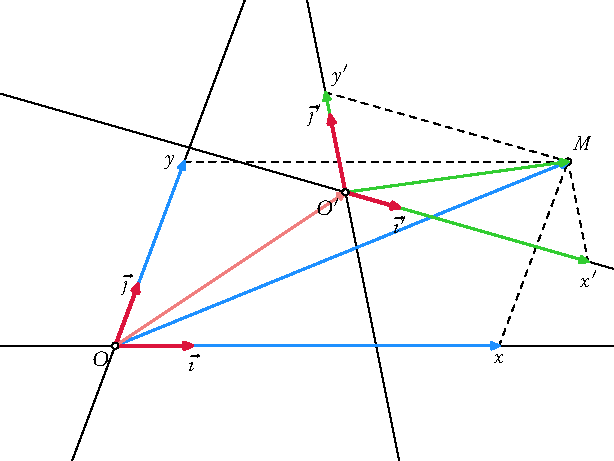
\includegraphics[scale=0.86]{figure.pdf}
}\hfill
\parbox{0.5\textwidth}{\Large\raggedleft
   \textbf{Contributeurs}\\
   Maxime \textsc{Chupin}\\
   Jean-Michel \textsc{Sarlat}
}
\vfill
\begin{center}
Version 1.1 du 22 octobre 2024\\
\url{https://gitlab.gutenberg-asso.fr/mchupin/mp-geom2d}\\
\url{https://ctan.org/pkg/mp-geom2d}
\end{center}
%% == Page de garde ====================================================
\newpage



\section{Objectif}

\mpgeomdd a été écrit avec le but de proposer des macros \MP{} permettant
de réaliser une figure de géométrie \emph{en collant} d'assez près
à une description impérative:
\begin{quote}\itshape
Soit \(A\) le point de coordonnées (2,3).\\
Soit \(B\) le point de coordonnées (4,5).\\
Trace la droite \((A,B)\).\\
....
\end{quote}
Dans ce cadre, les objets géométriques sont le plus souvent nommés
(\(A\), \(B\), etc.) ou désignés par leur nature et leurs attributs
(droite \((A,B)\), etc.). Pour ne pas avoir à dépasser ce mode de
description, en particulier pour éviter d'avoir à déclarer le
\emph{type} de ces objets, le choix a été fait de les identifier par
un \emph{index}\footnote{Le type \typeMP{numeric}, qui est le type par
défaut dans \MP, ne demande pas de déclaration préalable.} dans des
tables qui en précisent les caractéristiques.

\begin{Note} À ce jour, l'objectif n'est pas atteint, le
développement est loin d'être achevé; il est encore nécessaire de
faire appel à des commandes \MP{} ou à des \emph{macros
intermédiaires} pour décrire une figure. Cela évoluera sans doute
avec le temps, le temps de trouver une syntaxe satisfaisante...
\end{Note}


\section{Les fichiers}

\mpgeomdd est un ensemble d'outils pour la géométrie plane avec
\MP~\cite{ctan-metapost}. Cet 
ensemble est organisé en plusieurs fichiers :

\begin{enumerate}
\item \fichier{geom2d.mp} : c'est le fichier principal, qui charge tous les
autres ;
\item \fichier{geom2d-main.mp} : il contient
  les structures et fonctions générales ;
\item \fichier{geom2d-arc.mp} :
  contient tout ce qui concerne les arcs de cercles ;
\item \fichier{geom2d-c2d.mp} :
  contient tout ce qui concerne les courbes du second degré ;
\item \fichier{geom2d-fct.mp} :
  contient quelques fonctions mathématiques usuelles ;
\item \fichier{geom2d-lbl.mp} :
  contient les fonctions relatives aux labels ;
\item \fichier{geom2d-plt.mp} :
  contient des fonctions facilitant la représentation de fonctions
  mathématiques ;
\item \fichier{geom2d-rep.mp}
  contient différents outils pour le tracé de figure dans un repère ;
\item \fichier{geom2d-tra.mp}
  contient les fonctions permettant de gérer la transparence (code
  emprunté à Anthony \bsc{Phan}) ;
\item \fichier{geom2d-svgnames.mp} fournit les 150 couleurs de la spécification
SVG. 
\end{enumerate}

Nous allons, dans la suite, décrire plus en détails chacune de ces
fonctions. Certaines fonctions s'appuient sur
l'extension \fichier{graph.mp} présente dans toutes les bonnes
distributions \TeX.

\section{Principe général de fonctionnement}

\mpgeomdd utilise des tables comme structure principale. Chaque objet est
numéroté \emph{via} le compteur \variableGDD{gddO}, son type\footnote{Les types
sont propres à \mpgeomdd et seront décrits plus tard.} est stocké dans
la table \variableGDD{gddT[]} à la place \variableGDD{gddT[gddO]}. Les
propriétés des objets sont définies dans, là encore, des tables de
type \typeMP{numeric} qui sont \variableGDD{gddA[]}, \variableGDD{gddB[]},
\dots, \variableGDD{gddF[]}.

Par exemple, pour un \typeGDD{Point} (type \mpgeomdd), la première coordonnée
se trouve dans \variableGDD{gddA[]} et la seconde dans \variableGDD{gddB[]}
(les autres table ne sont pas utilisées pour un tel objet).

Il y a trois tables particulières \variableGDD{gddP[]} qui est du type
\typeMP{path}, \variableGDD{gddPX[][]} qui est sa version étendue, et \variableGDD{gddS[]} qui est du type
\typeMP{string}. Nous verrons plus tard quelle est leur utilité.

Bien entendu, lors d'une utilisation classique de \mpgeomdd, l'appel à
toutes ces tables n'est pas chose courante. Les fonctions que nous
allons décrire dans la suite de ce document permettent de ne pas
avoir recours trop précisément à cette machinerie.


\section{Tracés}

\mpgeomdd fournit des macros pour tracer des objets. Une commande permet de tracer
la plupart des objets de \mpgeomdd (qui sont décrits dans la
section~\ref{sec:types}), ainsi que certains type \MP. Les exemples tout au long
de la documentation permettront d'illustrer les commandes de tracé.

Pour comprendre comment fonctionne les représentations avec \mpgeomdd, il nous faut
tout d'abord décrire le mécanisme de gestion des unités.

\subsection{Unité}

\mpgeomdd définit une unité générale avec la variable globale
\lstinline+gddU+. Ce \typeMP{numeric} vaut par
défaut \SI{1}{cm}.
\begin{colourband}
  \macro|gddU|
  \index{gddU@\lstinline+gddU+}
  \end{colourband}
\subsection{En place}

Lors de l'utilisation des commandes de tracé, \mpgeomdd utilise la macro\label{gddEnPlace}
\begin{colourband}
\macro|gddEnPlace|
\index{gddEnPlace@\lstinline+gddEnPlace+}
\end{colourband}
Cette macro permet de spécifier les transformations géométriques nécessaires au
placement de l'objet, notamment le facteur d'échelle relatif à l'unité
\lstinline+gddU+.

En interne, cette macro est un \lstinline+scantoken+ de la variable globale
\variableGDD{gddW}\index{gddW@\lstinline+gddW+} (\typeMP{string}) qui contient les transformations. 

\subsection{Commandes de tracés}\label{sec:trace}

La macro de tracé la plus courante est la macro \lstinline+trace+.
\begin{colourband}
\macro|trace(«objet»)|
\begin{description}
  \item[\meta{objet}:] 
  \begin{itemize}
    \item pour le côté \MP, un \typeMP{path}, une
  \typeMP{picture} ou  un \typeMP{pair}, et dans ce cas \lstinline+trace+ sera
  équivalent à \lstinline+draw+;
    \item du côté de \mpgeomdd,
  n'importe quel des 6 objets définis jusque là : \typeGDD{triangle},
  \typeGDD{segment}, \typeGDD{droite}, \typeGDD{cercle}, \typeGDD{ellipse},
  \typeGDD{parabole}, \typeGDD{hyperbole},
  \typeGDD{polygone}, \typeGDD{chemin},
  \typeGDD{courbe} ou \typeGDD{vecteur} (pour ce dernier, une flèche sera
  ajoutée à l'extrémité du vecteur).
  \end{itemize}
\end{description}\index{trace@\lstinline+trace+}
\end{colourband}

Lorsque \lstinline+trace+ est utilisée sur un objet de \mpgeomdd, la macro fait
appel à la commande \MP\ \lstinline+draw+ avec le mécanisme de mise en place
décrit plus haut.

\mpgeomdd fournit un tracé avec flèche faisant non plus appel à \lstinline+draw+
mais à \lstinline+drawarrow+.

\begin{colourband}
\macro|fleche(«objet»)|
\begin{description}
  \item[\meta{objet}:] 
  \begin{itemize}
    \item pour le côté \MP, un \typeMP{path}, une
  \typeMP{picture} ou  un \typeMP{pair}, et dans ce cas \lstinline+trace+ sera
  équivalent à \lstinline+drawarrow+;
    \item du côté de \mpgeomdd,
  n'importe quel des 6 objets définis jusque là : \typeGDD{triangle},
  \typeGDD{segment}, \typeGDD{droite}, \typeGDD{cercle}, \typeGDD{ellipse},
  \typeGDD{polygone}, \typeGDD{chemin},
  \typeGDD{courbe} ou \typeGDD{vecteur} (pour ce dernier, une flèche sera
  ajoutée à l'extrémité du vecteur).
  \end{itemize}
\end{description}\index{fleche@\lstinline+fleche+}
\end{colourband}

On peut aussi colorier un objet grâce à la macro suivante.
\begin{colourband}
\macro|colorie(«objet»)|
\begin{description}
  \item[\meta{objet}:] peut être:
  \begin{itemize}
    \item pour le côté \MP, uniquement un \typeMP{path} et dans ce cas \lstinline+trace+ sera équivalent à \lstinline+fill+;
    \item du côté de \mpgeomdd,
  n'importe quel objet coloriable : \typeGDD{triangle},
   \typeGDD{cercle}, \typeGDD{ellipse}, \typeGDD{polygone}, \typeGDD{chemin}, ou
  \typeGDD{courbe}.
  \end{itemize}
\end{description}\index{colorie@\lstinline+colorie+}
\end{colourband}


Les commandes de tracés de \mpgeomdd font appel aux macros de
base de \MP : \lstinline+draw+ et \lstinline+fill+. Ainsi, pour spécifier la
couleur, on pourra
utiliser la commande \lstinline+withcolor+ ou bien la macro
\lstinline+drawoptions+.


On peut aussi colorier avec de la transparence\footnote{En réalité, on simule de
la transparence avec le code emprunté à Anthony Phan :
\url{http://www-math.univ-poitiers.fr/~phan/metalpha.html}} avec la commande
suivante.
\begin{colourband}
\macro|colorieAvecTransparence(«objet»,«couleur»,«coefficient de transparence»)|
\begin{description}
  \item[\meta{objet}:] peut être:
  \begin{itemize}
    \item pour le côté \MP, uniquement un \typeMP{path} et dans ce cas \lstinline+trace+ sera équivalent à \lstinline+fill+;
    \item du côté de \mpgeomdd,
  n'importe quel objet coloriable : \typeGDD{triangle},
   \typeGDD{cercle}, \typeGDD{ellipse}, \typeGDD{polygone}, \typeGDD{chemin}, ou
  \typeGDD{courbe}.
  \end{itemize}
  \item[\meta{couleur}:] est une \typeMP{color}.
  \item[\meta{coefficient de transparence}:] est un \typeMP{numeric} compris
  entre 0 et 1, 0 pour un coloriage opaque et 1 pour un coloriage invisible.
\end{description}\index{colorie@\lstinline+colorie+}
\end{colourband}




Les macros ci-dessus, font appel à une macro plus bas niveau qui permet de
retourner le \typeMP{path} à tracer ou colorier pour tous les objets \mpgeomdd.

\begin{colourband}
\macro|gddTraceObjet(«objet»)|\return{\typeMP{path}}
\begin{description}
  \item[\meta{objet}:]
   \typeGDD{triangle}, \typeGDD{segment}, \typeGDD{vecteur},
   \typeGDD{cercle}, \typeGDD{ellipse}, \typeGDD{parabole}, \typeGDD{hyperbole},\typeGDD{polygone}, \typeGDD{chemin}, ou
  \typeGDD{courbe}.
\end{description}\index{gddTraceObjet@\lstinline+gddTraceObjet+}
\end{colourband}

Si l'objet n'est pas fermé, \mpgeomdd fournit la macro suivante qui ajoute un
\lstinline+--cycle+ à la suite du chemin :
\begin{colourband}
\macro|fermeture(«objet»)|\return{\typeMP{path}}\indication{fermé \lstinline+--cycle+}
\begin{description}
  \item[\meta{objet}:]
  \begin{itemize}
    \item du côté de \MP, \typeMP{path} ;
    \item du côté de \mpgeomdd, \typeGDD{triangle}, \typeGDD{segment}, \typeGDD{vecteur},
   \typeGDD{cercle}, \typeGDD{chemin}, ou
  \typeGDD{courbe}.
  \end{itemize}
\end{description}\index{fermeture@\lstinline+fermeture+}
\end{colourband}

On pourra spécifier le \emph{crayon} utilisé pour les tracés avec la commande
suivante:

\begin{colourband}
  \macro|avecCrayon(«taille»,«couleur»)|
  \begin{description}
    \item[\meta{taille}:] facteur d'échelle \typeMP{numeric} du \typeMP{pen}
    \lstinline+pencircle+ de \MP{} utilisé ;
    \item[\meta{couleur}:] couleur \typeMP{color} à utiliser. 
  \end{description}\index{avecCrayon@\lstinline+avecCrayon+}
\end{colourband}
  
Cette macro est un raccourci pour le \emph{classique} \texttt{withpen
pencircle scaled ... withcolor ...}. On peut d'ailleurs évidemment toujours
utiliser les commandes \MP{} pour le dessin. 

On peut représenter les objets de type \typeGDD{point}. Pour cela, on dispose
d'une commande qui trace un petit cercle coloré à l'endroit du point. La
commande est la suivante :

\begin{colourband}
\macro|pointe(«point»)|
\begin{description}
  \item[\meta{point}:] \typeGDD{point} ou \typeMP{pair}
\end{description}\index{pointe@\lstinline+pointe+}
\end{colourband}

Cette macro utilise deux variables globales de \mpgeomdd qui sont
\begin{colourband}
\macro|gddTaillePoint|\indication{\typeMP{numeric}, valeur par défaut 3}
\index{gddTaillePoint@\lstinline+gddTaillePoint+}
\end{colourband}
et
\begin{colourband}
\macro|gddCouleurPoint| \indication{\typeMP{color}, valeur par défaut \lstinline+white+}
\index{gddCouleurPoint@\lstinline+gddCouleurPoint+}
\end{colourband}

Il existe deux autres types de pointage de point : la simple croix et le simple
disque. Pour choisir un autre type de pointage (en utilisant la même commande
\lstinline+pointe+), on modifiera la variable globale suivante:
\begin{colourband}
  \macro|gddPointType| \indication{\typeMP{string}, valeur par défaut
  \lstinline+"pointe"+}
  \par 

  Peut valoir : \lstinline+"pointe"+, \lstinline+"croix"+ ou \lstinline+"disque"+. 
  \index{gddPointType@\lstinline+gddPointType+}
\end{colourband}
\subsection{Contenir les tracés}

Il est souvent nécessaire de restreindre les tracés à une zone du plan $\R^2$.
Pour cela, \mpgeomdd fournit la commande \lstinline+Fenetre+:
\begin{colourband}
\macro|Fenetre(«Xmin»,«Ymin»,«Xmax»,«Ymin»)|
\index{Fenetre@\lstinline+Fenetre+}
\end{colourband}
Cette fonction trace un rectangle dont deux sommets opposés sont les points
\lstinline|(Xmin,Ymin)| et \lstinline|(Xmax,Ymax)| avec la couleur \MP{}
\lstinline+background+ et découpe l'image courante autour de ce cadre (avec la
commande \MP{} \lstinline+clip currentpicture+).


\section{Les types}\label{sec:types}

\mpgeomdd, fournit plusieurs types d'objets. Le type d'objet est
stocké dans la table \variableGDD{gddT[]}, et les tables \variableGDD{gddA[]}
à \variableGDD{gddF[]}, ainsi que la table \variableGDD{gddX} contiennent les propriétés des objets.

Nous allons ici décrire chaque type de l'extension \mpgeomdd,
leurs propriétés respectives, ainsi que des méthodes associées directement à
l'objet.

\subsection{Le type \typeGDD{point}}

Ce type correspond au point de
l'espace euclidien.

\subsubsection{Constructeur}

Pour être plus clair voici la fonction principale
pour créer un tel objet :
%
\begin{mpcode}
vardef Point(expr a,b) =
  gddT[incr gddO] = "point";
  gddA[gddO] = a; gddB[gddO] = b; gddO
enddef;
\end{mpcode}

\begin{colourband}
\macro|Point(«x»,«y»)|\return{\typeGDD{point}}
\begin{description}
  \item[\meta{x}:] \typeMP{numeric} ;
  \item[\meta{y}:] \typeMP{numeric}.
\end{description}\index{Point@\lstinline+Point+}
\end{colourband}
\bigskip


Cette fonction \og{}retourne\fg{} le compteur \variableGDD{gdd0} et crée dans la
table de type une entrée \typeGDD{point} et les attributs (coordonnées)
correspondants \variableGDD{a} et \variableGDD{b} dans les tables
\variableGDD{gddA} et \variableGDD{gddB}.

Avec un tel type de fonctionnement, la plupart des manipulations se
fait sur des \typeMP{numeric}s. En effet, pour déclarer un
\typeGDD{point}, il suffit d'écrire
\begin{mpcode}
A = Point(2,3);
\end{mpcode}
\variableGDD{A} prend alors la valeur courante de \variableGDD{gddO}. C'est
l'identifiant du point.

On peut aussi définir un \typeGDD{point} par ses coordonnées \emph{polaires}
avec la commande suivante.

\begin{colourband}
\macro|PointPolaire(«r»,«a»)|\return{\typeGDD{point}}
\begin{description}
  \item[\meta{r}:] \typeMP{numeric}, module du point;
  \item[\meta{a}:] \typeMP{numeric}, angle par rapport à l'axe des abscisses.
\end{description}\index{Point@\lstinline+Point+}
\end{colourband}
\bigskip



On peut définir un point dans un repère défini lui par un point
d'origine et deux vecteurs avec la fonction suivante:
\begin{colourband}
\macro|PointDansRepere(«x»,«y»,«o»,«i»,«j»)|\return{\typeGDD{point}}
\begin{description}
  \item[\meta{x}:] \typeMP{numeric} ;
  \item[\meta{y}:] \typeMP{numeric} ;
  \item[\meta{o}:] \typeGDD{point} d'origine du repère ;
  \item[\meta{i}:] \typeGDD{vecteur} (ou \typeGDD{point}) définissant l'axe des abscisses ;
  \item[\meta{j}:] \typeGDD{vecteur} (ou \typeGDD{point}) définissant l'axe des ordonnées.
\end{description}\index{PointDansRepere@\lstinline+PointDansRepere+}
\end{colourband}

\bigskip

Le code suivant illustre l'utilisation de cette commande (avec des
\typeGDD{point}s au lieu de \typeGDD{vecteur}s, type décrit plus tard). 
\begin{mpcode}
O = Point(0,0);
I = Point(2,0);
J = Point(0,3);
A = PointDansRepere(2,3,O,I,J);
\end{mpcode}


\subsubsection{Macros associées}

On peut récupérer l'abscisse et l'ordonnée d'un point avec les commandes
suivantes :
\begin{colourband}
\macro|Abscisse(«a»)|\return{\typeMP{numeric}}
\begin{description}
  \item[\meta{a}:] \typeGDD{point}, \typeGDD{vecteur} ou \typeMP{pair}.
\end{description}\index{Abscisse@\lstinline+Abscisse+}
\end{colourband}

\begin{colourband}
\macro|Ordonnee(«a»)|\return{\typeMP{numeric}}
\begin{description}
  \item[\meta{a}:] \typeGDD{point}, \typeGDD{vecteur} ou \typeMP{pair}.
\end{description}\index{Ordonnee@\lstinline+Ordonnee+}
\end{colourband}

On pourra ajouter les abscisses, les ordonnées ou bien, à la manière des
vecteurs, des points entre eux avec les commandes suivantes.
\begin{colourband}
\macro|AdditionAbscisses(«a»)|\return{\typeMP{numeric}}
\begin{description}
  \item[\meta{a}:] \typeGDD{point} ou \typeMP{pair}.
\end{description}\index{AdditionAbscisses@\lstinline+AdditionAbscisses+}
\end{colourband}
\begin{colourband}
\macro|AdditionOrdonnee(«a»)|\return{\typeMP{numeric}}
\begin{description}
  \item[\meta{a}:] \typeGDD{point} ou \typeMP{pair}.
\end{description}\index{AdditionOrdonnee@\lstinline+AdditionOrdonnee+}
\end{colourband}
et
\begin{colourband}
\macro|Addition(«a»,«b»)|\return{\typeGDD{point}}
\begin{description}
  \item[\meta{a}:] \typeGDD{point} ou \typeMP{pair};
  \item[\meta{b}:] \typeGDD{point} ou \typeMP{pair}.
\end{description}\index{Addition@\lstinline+Addition+}
\end{colourband}

On peut aussi calculer la longueur entre deux points grâce à la commande
suivante:
\begin{colourband}
\macro|Longueur(«a»,«b»)|\return{\typeMP{numeric}}
\begin{description}
  \item[\meta{a}:] \typeGDD{point} ou \typeMP{pair};
  \item[\meta{b}:] \typeGDD{point} ou \typeMP{pair}.
\end{description}\index{Longueur@\lstinline+Longueur+}
\end{colourband}

On peut calculer le point équidistant de deux points, le milieu :
\begin{colourband}
\macro|Milieu(«a»,«b»)|\return{\typeGDD{point}}
\begin{description}
  \item[\meta{a}:] \typeGDD{point} ou \typeMP{pair};
  \item[\meta{b}:] \typeGDD{point} ou \typeMP{pair}.
\end{description}\index{Milieu@\lstinline+Milieu+}
\end{colourband}

On peut réaliser la rotation d'un point autour de l'origine $(0,0)$ avec la
commande suivante:
\begin{colourband}
\macro|Rotation(«a»,«b»)|\return{\typeGDD{point}}
\begin{description}
  \item[\meta{a}:] \typeGDD{point} ou \typeMP{pair};
  \item[\meta{b}:] \typeMP{numeric}, l'angle de rotation en radian.
\end{description}\index{Rotation@\lstinline+Rotation+}
\end{colourband}

Si on veut réaliser la rotation d'un point autour d'un autre, on utilisera la
commande suivante:
\begin{colourband}
\macro|RotationCentre(«a»,«b»,«c»)|\return{\typeGDD{point}}
\begin{description}
  \item[\meta{a}:] \typeGDD{point} ou \typeMP{pair};
  \item[\meta{b}:] \typeGDD{point} ou \typeMP{pair}, centre de rotation;
  \item[\meta{c}:] \typeMP{numeric}, l'angle de rotation en radian.
\end{description}\index{RotationCentre@\lstinline+RotationCentre+}
\end{colourband}

On peut calculer l'isobarycentre d'une liste de points (ou de \typeMP{pair} de \MP) avec la commande suivante.
\begin{colourband}
\macro|IsoBarycentre(«a»,«b»,«c», etc.)|\return{\typeGDD{point}}
\begin{description}
  \item[\meta{a}:] \typeGDD{point} ou \typeMP{pair};
  \item[\meta{b}:] \typeGDD{point} ou \typeMP{pair} ;
  \item[] etc.
\end{description}\index{IsoBarycentre@\lstinline+IsoBarycentre+}
\end{colourband}

On peut calculer le barycentre d'une liste de points associées à des poids (mais
ici, il n'est pas possible d'utiliser des \typeMP{pair} de \MP).
\begin{colourband}
\macro|Barycentre((«A»,«a»),(«B»,«b»),(«C»,«c»), etc.)|\return{\typeGDD{point}}
\begin{description}
  \item[\meta{A}:] \typeGDD{point} ;
  \item[\meta{a}:] \typeMP{numeric}, poids associé à \meta{A} ;
  \item[\meta{B}:] \typeGDD{point} ;
  \item[\meta{b}:] \typeMP{numeric}, poids associé à \meta{B} ;
  \item[] etc.
\end{description}\index{Barycentre@\lstinline+Barycentre+}
\end{colourband}


On peut déterminer la bissectrice d'un secteur angulaire défini par trois
points. La fonction retourne une \typeGDD{droite}.
\begin{colourband}
\macro|Bissectrice(«A»,«B»,«C»)|\return{\typeGDD{droite}}
\begin{description}
  \item[\meta{A}:] \typeGDD{point} ;
  \item[\meta{B}:] \typeGDD{point} ;
  \item[\meta{C}:] \typeGDD{point}.
\end{description}\index{Bissectrice@\lstinline+Bissectrice+}
\end{colourband}

\begin{ExempleMP}
input geom2d;
beginfig(1);
A = Point(1,0);
B = Point(0,0);
C = Point(1,1);
D = Bissectrice(A,B,C);
trace D;
marque.bot "A";
marque.bot "B";
marque.bot "C";
Fenetre(-0.5,-0.5,2,2);
endfig;
\end{ExempleMP}


Le type \typeGDD{point} est évidemment lié au type \MP{} \typeMP{pair}.

\mpgeomdd fournit des macros qui permettent de passer de \typeGDD{point} à
\typeMP{pair} et réciproquement.
\begin{colourband}
\macro|PointTOPair(«a»,«b»)|\return{\typeMP{pair}}
\begin{description}
  \item[\meta{a}:] \typeMP{numeric}, abscisse ;
  \item[\meta{b}:] \typeMP{numeric}, ordonnée.
\end{description}\index{PointTOPair@\lstinline+PointTOPair+}
\end{colourband}


\begin{colourband}
\macro|PairTOPoint(«p»)|\return{\typeGDD{point}}
\begin{description}
  \item[\meta{p}:] \typeMP{pair}.
\end{description}\index{PairTOPoint@\lstinline+PairTOPoint+}
\end{colourband}

Ces deux commandes sont complétées par deux autres qui assure qu'un élément est
d'un type donné:
\begin{colourband}
\macro|PairImp(«p»)|\return{\typeGDD{pair}}
\begin{description}
  \item[\meta{p}:] \typeGDD{point} ou \typeMP{pair}.
\end{description}\index{PairImp@\lstinline+PairImp+}
\end{colourband}


\begin{colourband}
\macro|PointImp(«p»)|\return{\typeGDD{point}}
\begin{description}
  \item[\meta{p}:] \typeGDD{point} ou \typeMP{pair}.
\end{description}\index{PointImp@\lstinline+PointImp+}
\end{colourband}

On peut aussi récupérer un point le long d'un objet \mpgeomdd (décrit dans les
sections suivantes). La macro suivante retourne un \typeGDD{point} le long du
chemin (cyclique ou non) de l'objet le paramétrant entre 0 et 1.

\begin{colourband}
\macro|PointDe(«o»,«t»)|\return{\typeGDD{point}}
\begin{description}
  \item[\meta{o}:] n'importe quel objet \mpgeomdd (même un \typeGDD{point} pour
  lequel lui-même est retourné);
  \item[\meta{t}:] \typeMP{numeric} compris entre 0 et 1 (qui paramètre le
  chemin de l'objet entre 0 et 1).
\end{description}\index{PointDe@\lstinline+PointDe+}
\end{colourband}



\subsection{Le type \typeGDD{vecteur}}

Ce type correspond aux vecteurs
définis à l'aide de deux coordonnées de l'espace euclidien.

\subsubsection{Constructeurs}

La fonction
créatrice d'un tel objet est celle-ci
%
\begin{mpcode}
vardef Vecteur(expr a,b) =
  save n; n = incr gddO;
  gddT[n] = "vecteur"; gddA[n] = a; gddB[n] = b; n
enddef;
\end{mpcode}

\begin{colourband}
\macro|Vecteur(«a»,«b»)|\return{\typeGDD{vecteur}}
\begin{description}
  \item[\meta{a}:] \typeMP{numeric} ;
  \item[\meta{b}:] \typeMP{numeric}.
\end{description}\index{Vecteur@\lstinline+Vecteur+}
\end{colourband}
\bigskip

Cette fonction a la même architecture que celle correspondante au
\typeGDD{point} : elle retourne la valeur courante de \variableGDD{gddO}
après incrémentation, puis affecte le type \typeGDD{vecteur} à
l'entrée correspondante dans la table \variableGDD{gddT}.

On peut aussi définir un vecteur à partir d'un \typeMP{pair} \MP.
\begin{mpcode}
vardef VecteurP(expr a) =
  save n; n = incr gddO;
  gddT[n] = "vecteur"; gddA[n] = xpart a; gddB[n] = ypart a; n
enddef;
\end{mpcode}

\begin{colourband}
\macro|VecteurP(«a»)|\return{\typeGDD{vecteur}}
\begin{description}
  \item[\meta{a}:] \typeMP{pair}.
\end{description}\index{VecteurP@\lstinline+VecteurP+}
\end{colourband}
\bigskip

Un vecteur peut se définir alors comme ceci:
\begin{ExempleMP}
input geom2d;
beginfig(1);
AB = Vecteur(2,3);
pair a;
a := (3,2);
A = VecteurP(a);
trace AB;
trace A;
endfig;
\end{ExempleMP}

\subsubsection{Macros associées}

Comme les objets de \mpgeomdd ne sont pas des \typeMP{numeric}s, les opérations classiques
de l'espace vectoriel ne peuvent pas s'écrire avec les simples caractères
\lstinline-+-, \lstinline+-+, et \lstinline-*-.

\begin{colourband}
\macro|AdditionVecteur(«a»,«b»)|\return{\typeGDD{vecteur}}
\begin{description}
  \item[\meta{a}:] \typeGDD{vecteur} ;
  \item[\meta{b}:] \typeGDD{vecteur}.
\end{description}\index{AdditionVecteur@\lstinline+AdditionVecteur+}
\end{colourband}
\bigskip


\begin{colourband}
\macro|SoustractionVecteur(«a»,«b»)|\return{\typeGDD{vecteur}}
\begin{description}
  \item[\meta{a}:] \typeGDD{vecteur} ;
  \item[\meta{b}:] \typeGDD{vecteur}.
\end{description}\index{SoustractionVecteur@\lstinline+SoustractionVecteur+}
\end{colourband}
\bigskip


\begin{colourband}
\macro|ScalaireVecteur(«k»,«b»)|\return{\typeGDD{vecteur}}
\begin{description}
  \item[\meta{k}:] \typeMP{numeric} ;
  \item[\meta{b}:] \typeGDD{vecteur}.
\end{description}\index{ScalaireVecteur@\lstinline+ScalaireVecteur+}
\end{colourband}
\bigskip

On pourra alors faire les opérations classiques sur les vecteurs.

\begin{ExempleMP}
input geom2d;
beginfig(1);
AB = Vecteur(2,3);
BC = Vecteur(1,0);
AC = AdditionVecteur(AB,BC);
kAC = ScalaireVecteur(3.0,AC);
trace AB;
trace BC;
trace AC;
endfig;
\end{ExempleMP}

On peut aussi calculer le produit scalaire de deux vecteurs avec la commande
suivante.

\begin{colourband}
\macro|ProduitScalaire(«a»,«b»)|\return{\typeMP{numeric}}
\begin{description}
  \item[\meta{a}:] \typeGDD{vecteur} ;
  \item[\meta{b}:] \typeGDD{vecteur}.
\end{description}\index{ProduitScalaire@\lstinline+ProduitScalaire+}
\end{colourband}
\bigskip

On peut aussi calculer la norme euclidienne d'un vecteur.
\begin{colourband}
\macro|Norme(«a»)|\return{\typeMP{numeric}}
\begin{description}
  \item[\meta{a}:] \typeGDD{vecteur}.
\end{description}\index{Norme@\lstinline+Norme+}
\end{colourband}
\bigskip

La commande suivante permet d'obtenir l'angle, en radian, entre $[0,\uppi]$ formé
entre deux vecteurs. Si on note $u$ et $v$ les deux vecteurs de $\R^2$, l'angle
calculé par la commande suivante est obtenu avec la formule suivante :
\[\theta = \arccos \left(\frac{u\cdot v}{\|u\|\|v\|}\right).\]

\begin{colourband}
\macro|Angle(«a»,«b»)|\return{\typeMP{numeric} (dans $[0,\uppi]$)}
\begin{description}
  \item[\meta{a}:] \typeGDD{vecteur} ;
  \item[\meta{b}:] \typeGDD{vecteur}.
\end{description}\index{Norme@\lstinline+Norme+}
\end{colourband}
\bigskip


\subsection{Le type \typeGDD{segment}}
Les segments sont
définis par deux points de $\R^2$.


\subsubsection{Constructeur}
La fonction créatrice de cet objet est
celle-ci
\begin{mpcode}
vardef Segment (expr a,b) =
  save n; n = incr gddO;
  gddT[n] = "segment"; gddA[n] = PointImp(a); gddB[n] = PointImp(b); n
enddef;
\end{mpcode}

\begin{colourband}
\macro|Segment(«a»,«b»)|\return{\typeGDD{segment}}
\begin{description}
  \item[\meta{a}:]  \typeGDD{point} ;
  \item[\meta{b}:]  \typeGDD{point}.
\end{description}\index{Segment@\lstinline+Segment+}
\end{colourband}

\bigskip

Un segment se définit alors comme ceci:
\begin{ExempleMP}
input geom2d;
beginfig(1);
A = Point(2,3);
B = Point(4,5);
C = Point(2,1);
AB = Segment(A,B);
BC = Segment(B,C);
AC = Segment(A,C);
fleche AB;
fleche BC;
fleche AC;
endfig;
\end{ExempleMP}

\subsubsection{Macros associées}

On peut calculer la longueur d'un segment avec la macro suivante.
\begin{colourband}
\macro|LongueurSegment(«a»)|\return{\typeMP{numeric}}
\begin{description}
  \item[\meta{a}:]  \typeGDD{segment}.
\end{description}\index{LongueurSegment@\lstinline+LongueurSegment+}
\end{colourband}

On peut aussi convertir un segment en vecteur avec la macro suivante qui fait la
différence des coordonnées des deux points définissant le segment.
\begin{colourband}
\macro|SegmentTOVecteur(«a»)|\return{\typeGDD{vecteur}}
\begin{description}
  \item[\meta{a}:]  \typeGDD{segment}.
\end{description}\index{SegmentTOVecteur@\lstinline+SegmentTOVecteur+}
\end{colourband}



\subsection{Le type \typeGDD{droite}}
Une droite est simplement définie par
deux points.

\subsubsection{Constructeur}

Ainsi la fonction créatrice de cet objet est la suivante
\begin{mpcode}
vardef Droite (expr a,b) =
  save n; n = incr gddO;
  gddT[n] = "droite"; gddA[n] = PointImp(a); gddB[n] = PointImp(b); n
enddef;
\end{mpcode}
\begin{colourband}
\macro|Droite(«a»,«b»)|\return{\typeGDD{droite}}
\begin{description}
  \item[\meta{a}:]  \typeGDD{point} ;
  \item[\meta{b}:]  \typeGDD{point}.
\end{description}\index{Droite@\lstinline+Droite+}
\end{colourband}
\bigskip

Lors de la représentation des droites (voir section~\ref{sec:trace}), le
caractère \emph{infini} de la droite est géré par la variable globale
\lstinline+gddExtensionDroite+ 
\index{gddExtensionDroite@\lstinline+gddExtensionDroite+}
qui vaut 10 par défaut.

\subsubsection{Macros associées}


La macro suivante permet, sous forme d'un triplet, et donc d'une \typeMP{color},
d'obtenir les coefficients d'une droite donnée. Pour une droite $(D)$, la macro
donne le triplet $(u,v,w)\in\R^3$ tel que $\forall (x,y)\in(D)$, $ux+vy+w=0$.

\begin{colourband}
\macro|EquationDroite(«a»)|\return{\typeMP{color}}
\begin{description}
  \item[\meta{a}:]  \typeGDD{droite}.
\end{description}\index{EquationDroite@\lstinline+EquationDroite+}
\end{colourband}

On peut calculer la projection d'un point sur une droite avec la commande
suivante.

\begin{colourband}
\macro|ProjectionPointSurDroite(«p»,«a»)|\return{\typeGDD{point}}
\begin{description}
  \item[\meta{p}:] \typeGDD{point} ;
  \item[\meta{a}:]  \typeGDD{droite}.
\end{description}\index{ProjectionPointSurDroite@\lstinline+ProjectionPointSurDroite+}
\end{colourband}

On peut obtenir l'ordonnée relative d'un point sur une droite avec la macro
suivante.
\begin{colourband}
\macro|OrdonneeRelativePointDroite(«p»,«a»)|\return{\typeMP{numeric}}
\begin{description}
  \item[\meta{p}:] \typeGDD{point} ;
  \item[\meta{a}:]  \typeGDD{droite}.
\end{description}\index{OrdonneeRelativePointDroite@\lstinline+OrdonneeRelativePointDroite+}
\end{colourband}

Le calcul de la distance d'un point à une droite se fait avec la macro suivante.
\begin{colourband}
\macro|DistancePointDroite(«p»,«a»)|\return{\typeMP{numeric}}
\begin{description}
  \item[\meta{p}:] \typeGDD{point} ;
  \item[\meta{a}:]  \typeGDD{droite}.
\end{description}\index{DistancePointDroite@\lstinline+DistancePointDroite+}
\end{colourband}

La macro suivante permet d'obtenir la droite perpendiculaire à un droite passant
par un point.
\begin{colourband}
\macro|DroitePerpendiculaire(«a»,«p»)|\return{\typeGDD{droite}}
\begin{description}
  \item[\meta{a}:]  \typeGDD{droite} ;
  \item[\meta{p}:] \typeGDD{point}.
\end{description}\index{DroitePerpendiculaire@\lstinline+DroitePerpendiculaire+}
\end{colourband}

On pourra obtenir le \typeGDD{point} d'intersection de deux droites avec la
macro suivante.
\begin{colourband}
\macro|IntersectionDroites(«a»,«b»)|\return{\typeGDD{point}}
\begin{description}
  \item[\meta{a}:]  \typeGDD{droite} ;
  \item[\meta{b}:] \typeGDD{droite}.
\end{description}\index{IntersectionDroites@\lstinline+IntersectionDroites+}
\end{colourband}

La macro suivante permet de reporter un point sur une droite avec une certaine
longueur (signée), à la manière d'un compas. 

\begin{colourband}
\macro|ReportSurDroite(«P»,«D»,«l»)|\return{\typeGDD{point}}
\begin{description}
  \item[\meta{P}:]  \typeGDD{point} ;
  \item[\meta{D}:] \typeGDD{droite} ;
  \item[\meta{l}:] \typeMP{numeric} (peut être négatif).
\end{description}\index{ReportSurDroite@\lstinline+ReportSurDroite+}
\end{colourband}

Le côté du report par rapport au point \meta{P} dépend de la définition de 
la droite : pour une droite définie par deux \typeGDD{point}s $A$ et $B$, alors
la direction du report sera suivant le vecteur $\overrightarrow{AB}$. Pour
changer de direction, il suffira de multiplier le paramètre de distance \meta{l}
par $-1$. 

Voici un exemple permettant d'illustrer l'utilisation de quelques commandes
relatives aux droites.

\begin{ExempleMP}
input geom2d;
beginfig(1);
A = Point(0,0);
B = Point(3,2);
AB = Droite(A,B);
trace AB;
pointe A;
pointe B;
C = Point(0,2);
DC = DroitePerpendiculaire(AB,C);
trace DC;
pointe C;
D = ProjectionPointSurDroite(C,AB);
pointe D;
Fenetre(-2,-2,4,4);
endfig;
\end{ExempleMP}





\subsection{Le type \typeGDD{cercle}}
Un cercle est défini par un point et un
rayon.

\subsubsection{Constructeurs}
La fonction créatrice de base de cet objet est la suivante
\begin{mpcode}
vardef Cercle (expr a,b) =
    save n; n = incr gddO;
    gddT[n] = "cercle"; gddA[n] = PointImp(a); gddB[n] = b; n
enddef;
\end{mpcode}
\begin{colourband}
\macro|Cercle(«a»,«b»)|\return{\typeGDD{cercle}}
\begin{description}
  \item[\meta{a}:]  \typeGDD{point} ou \typeMP{pair},
  centre du cercle ;
  \item[\meta{b}:] \typeMP{numeric}, rayon du cercle.
\end{description}\index{Cercle@\lstinline+Cercle+}
\end{colourband}
\bigskip


Deux autres fonctions permettent de définir des cercles. La fonction
\foncGDD{CercleCP} définit le cercle par un centre et un point par lequel passe
le cercle.
\begin{colourband}
\macro|CercleCP(«a»,«b»)|\return{\typeGDD{cercle}}
\begin{description}
  \item[\meta{a}:]  \typeGDD{point} ou \typeMP{pair},
  centre du cercle ;
  \item[\meta{b}:]  \typeGDD{point},
  tel que \meta{b}$-$\meta{a} est le rayon.
\end{description}\index{CercleCP@\lstinline+CercleCP+}
\end{colourband}
\bigskip



On peut aussi définir un cercle par deux points définissant son diamètre. La
fonction correspondante est la suivante

\begin{colourband}
\macro|CercleD(«a»,«b»)|\return{\typeGDD{cercle}}
\begin{description}
  \item[\meta{a}:]  \typeGDD{point} ou \typeMP{pair} ;
  \item[\meta{b}:]  \typeGDD{point} ou \typeMP{pair},
  tel que $($\meta{a}$-$\meta{b}$)$ est le diamètre du cercle.
\end{description}\index{CercleD@\lstinline+CercleD+}
\end{colourband}
\bigskip

On peut aussi définir un cercle comme le cercle qui passe par trois points avec
la macro suivante.

\begin{colourband}
\macro|CercleTroisPoints(«a»,«b»,«c»)|\return{\typeGDD{cercle}}
\begin{description}
  \item[\meta{a}:]  \typeGDD{point} ou \typeMP{pair} ;
  \item[\meta{b}:]  \typeGDD{point} ou \typeMP{pair} ;
  \item[\meta{c}:]  \typeGDD{point} ou \typeMP{pair}.
\end{description}\index{CercleTroisPoints@\lstinline+CercleTroisPoints+}
\end{colourband}
\bigskip




\begin{ExempleMP}
input geom2d;
beginfig(1);
A = Point(3,1);
B = Point(0,2);
O = Point(0,0);
r = 1.0;
COr = Cercle(O,r);
COA = CercleCP(O,A);
CAB = CercleD(A,B);
COAB = CercleTroisPoints(O,A,B);
trace COr;
trace COA;
trace CAB;
trace COAB;
pointe A; pointe B; pointe O;
endfig;
\end{ExempleMP}

\subsubsection{Macros associées}

De nombreuses macros sont associées aux cercles.

On pourra récupérer le rayon d'un cercle avec la commande suivante.


\begin{colourband}
\macro|Rayon(«a»)|\return{\typeMP{numeric}}
\begin{description}
  \item[\meta{a}:]  \typeGDD{cercle}.
\end{description}\index{Rayon@\lstinline+Rayon+}
\end{colourband}
\bigskip

On pourra obtenir le centre (\typeGDD{point}) d'un cercle avec la commande :
\begin{colourband}
\macro|Centre(«a»)|\return{\typeGDD{point}}
\begin{description}
  \item[\meta{a}:]  \typeGDD{cercle}, \typeGDD{ellipse} ou \typeGDD{hyperbole}.
\end{description}\index{Centre@\lstinline+Centre+}
\end{colourband}
\bigskip

On peut calculer l'intersection entre deux cercles grâce à la macro suivante.

\begin{colourband}
\macro|IntersectionCercles(«a»,«b»)|\return{\typeGDD{point}}
\begin{description}
  \item[\meta{a}:]  \typeGDD{cercle} ;
  \item[\meta{b}:]  \typeGDD{cercle}.
\end{description}\index{IntersectionCercles@\lstinline+IntersectionCercles+}
\end{colourband}
\bigskip

Cette macro ne donnera qu'un seul point d'intersection. Pour obtenir les deux
points d'intersection, il faudra inverser l'ordre d'appel sur les cercles comme
l'exemple suivant l'illustre.

\begin{ExempleMP}
input geom2d;
beginfig(1);
A = Point(0,0);
CA = Cercle(A,1);
B = Point(1.5,0);
CB = Cercle(B,2);
D1 = IntersectionCercles(CA,CB);
D2 = IntersectionCercles(CB,CA);
trace CA; trace CB;
pointe A; pointe B;  pointe D1; pointe D2;
endfig;
\end{ExempleMP}

Si il n'existe pas d'intersection, alors la compilation échouera avec l'erreur
\texttt{! Pythagorean subtraction X.XXXX+-+X.XXXX has been replaced by 0}. Si
les deux cercles sont confondus, alors l'erreur sera \texttt{! Division by zero.}.

\mpgeomdd fournit aussi une macro permettant d'obtenir les intersections entre une
droite et un cercle.

\begin{colourband}
\macro|IntersectionDroiteCercle(«d»,«c»,«n»)|\return{\typeGDD{point}}
\begin{description}
  \item[\meta{d}:]  \typeGDD{droite} ;
  \item[\meta{c}:]  \typeGDD{cercle} ;
  \item[\meta{n}:] \typeMP{numeric} qui vaut 1 ou 2 suivant le point
  d'intersection que l'on souhaite (s'il n'existe qu'un point d'intersection
  alors les deux valeurs renvoient le même point).
\end{description}\index{IntersectionDroiteCercle@\lstinline+IntersectionDroiteCercle+}
\end{colourband}
\bigskip

S'il n'existe pas d'intersection entre la droite et le cercle, vous obtiendrez
l'erreur \texttt{! Intersection between line and circle does not exist}.

L'exemple suivant permet d'illuster cette macro.
\begin{ExempleMP}
input geom2d;
beginfig(1);
A = Point(2,2);
C_A = Cercle(A,1);
B = Point(0,1);
C = Point(4,2);
BC = Droite(B,C);
E1 = IntersectionDroiteCercle(BC,C_A,1);
trace C_A;
trace BC dashed evenly;
pointe A; pointe B; pointe C; pointe E1;
Fenetre(-0.5,-0.5,5,4);
endfig;
\end{ExempleMP}



On peut obtenir les tangentes intérieures et extérieures communes à deux cercles
avec les deux macros suivantes. Là encore, comme il existe deux tangentes, pour
obtenir les deux, on inversera l'ordre d'appel des deux cercles.

\begin{colourband}
\macro|TangenteCommuneExterieure(«a»,«b»)|\return{\typeGDD{droite}}
\begin{description}
  \item[\meta{a}:]  \typeGDD{cercle} ;
  \item[\meta{b}:]  \typeGDD{cercle}.
\end{description}\index{TangenteCommuneExterieure@\lstinline+TangenteCommuneExterieure+}
\end{colourband}
\bigskip


\begin{colourband}
\macro|TangenteCommuneInterieure(«a»,«b»)|\return{\typeGDD{droite}}
\begin{description}
  \item[\meta{a}:]  \typeGDD{cercle} ;
  \item[\meta{b}:]  \typeGDD{cercle}.
\end{description}\index{TangenteCommuneInterieure@\lstinline+TangenteCommuneInterieure+}
\end{colourband}
\bigskip

L'exemple suivante illustre l'utilisation de ces deux macros.
\begin{ExempleMP}[sidebyside=false]
input geom2d;
beginfig(1);
C1 = Cercle((-2,0),2);
C2 = Cercle((1.5,0),1);
T1 = TangenteCommuneExterieure(C1,C2);
T2 = TangenteCommuneExterieure(C2,C1);
T3 = TangenteCommuneInterieure(C1,C2);
T4 = TangenteCommuneInterieure(C2,C1);
trace C1; trace C2;
trace T1; trace T2;
trace T3; trace T4;

Fenetre(-5,-3,6,3);
endfig;
\end{ExempleMP}

La macro suivante permet de calculer l'axe radical (\typeGDD{droite}) de deux
cercles\footnote{La méthode de construction a été largement inspirée du code de
T.~Thurston dans son document \emph{Drawing with \MP}~\cite{ctan-drawing-with-metapost}.}.
\begin{colourband}
\macro|AxeRadical(«a»,«b»)|\return{\typeGDD{droite}}
\begin{description}
  \item[\meta{a}:]  \typeGDD{cercle} ;
  \item[\meta{b}:]  \typeGDD{cercle}.
\end{description}\index{AxeRadical@\lstinline+AxeRadical+}
\end{colourband}
\bigskip

La macro suivante permet d'obtenir le centre radical de trois cercles.
\begin{colourband}
\macro|CentreRadical(«a»,«b»,«c»)|\return{\typeGDD{point}}
\begin{description}
  \item[\meta{a}:]  \typeGDD{cercle} ;
  \item[\meta{b}:]  \typeGDD{cercle} ;
  \item[\meta{c}:]  \typeGDD{cercle}.
\end{description}\index{CentreRadical@\lstinline+CentreRadical+}
\end{colourband}
\bigskip

La macro suivante permet de calculer l'axe de similitude de trois cercles.
\begin{colourband}
\macro|AxeDeSimilitude(«a»,«b»,«c»)|\return{\typeGDD{droite}}
\begin{description}
  \item[\meta{a}:]  \typeGDD{cercle} ;
  \item[\meta{b}:]  \typeGDD{cercle} ;
  \item[\meta{c}:]  \typeGDD{cercle}.
\end{description}\index{AxeDeSimilitude@\lstinline+AxeDeSimilitude+}
\end{colourband}
\bigskip

\subsection{Le type \typeGDD{ellipse}}
\subsubsection{Constructeurs}

Les ellipses peuvent être définies de plusieurs façons. Tout d'abord, on peut la
définir avec son centre, un des points de l'ellipse sur le grand axe (appelé
vertex), et un des points de l'ellipse sur le petit axe (appelé co-vertex).
Cependant, lors de la création d'une ellipse de nombreux attributs sont calculés.

Le code du contructeur est le suivant:
\begin{mpcode}
vardef Ellipse(expr C,A,B) =
  % C : centre
  % A : vertex
  % B : co-vertex
  save n,a,b,c,e,_tmp,slope;
  pair _tmp;
  n = incr gddO;
  gddT[n] = "ellipse"; gddA[n] = PointImp(C); gddB[n] = PointImp(A);
  gddC[n] = PointImp(B);
  % calcul des deux foyers
  a = Longueur(C,A);
  b = Longueur(C,B);
  c = sqrt(a**2-b**2);
  e = c/a;
  _tmp = e*(Pt(A)-Pt(C));
  % les foyers
  gddD[n] = PairTOPoint(Pt(C)+_tmp);
  gddE[n] = PairTOPoint(Pt(C)-_tmp);
  gddX[n][1] = a;
  gddX[n][2] = b;
  gddX[n][3] = e;
  % angle du demi-grand axe
  slope = angle(PairImp(A)-PairImp(C));
  gddX[n][4] = slope;
  n
enddef;
\end{mpcode}

\begin{colourband}
\macro|Ellipse(«c»,«a»,«b»)|\return{\typeGDD{ellipse}}
\begin{description}
  \item[\meta{c}:]  \typeGDD{point} ou \typeMP{pair}, le centre ;
  \item[\meta{a}:]  \typeGDD{point} ou \typeMP{pair}, le vertex ;
  \item[\meta{b}:]  \typeGDD{point} ou \typeMP{pair}, le co-vertex.
\end{description}\index{Ellipse@\lstinline+Ellipse+}
\end{colourband}
\bigskip

Cette macro s'utilise comme le montre l'exemple suivant.
\begin{ExempleMP}
input geom2d;
beginfig(1);
C = Point(0,0);
A = Point(3,1);
B = Rotation((1.5,0.5),Pi/2);
E = Ellipse(C,A,B);
trace E;
pointe A; pointe B; pointe C;
endfig;
\end{ExempleMP}

On pourra définir une ellipse avec la donnée de ses deux foyers et du 
demi-grand axe avec la commande suivante:
\begin{colourband}
\macro|EllipseF(«A»,«B»,«a»)|\return{\typeGDD{ellipse}}
\begin{description}
  \item[\meta{A}:]  \typeGDD{point} ou \typeMP{pair}, premier foyer ;
  \item[\meta{B}:]  \typeGDD{point} ou \typeMP{pair}, deuxième foyer ;
  \item[\meta{a}:]  \typeGDD{numeric}, le demi-grand axe.
\end{description}\index{EllipseF@\lstinline+EllipseF+}
\end{colourband}
\bigskip


Cette macro s'utilise comme le montre l'exemple suivant.
\begin{ExempleMP}
input geom2d;
beginfig(1);
F1 = Point(3,1);
F2 = Point(1.5,0.5);
E = EllipseF(F1,F2,1.7);
trace E;
pointe F1; pointe F2;
endfig;
\end{ExempleMP}

\subsubsection{Macros associées}

On pourra obtenir le centre (\typeGDD{point}) d'une ellipse avec la commande :
\begin{colourband}
  \macro|Centre(«a»)|\return{\typeGDD{point}}
  \begin{description}
    \item[\meta{a}:]  \typeGDD{cercle}, \typeGDD{ellipse} ou \typeGDD{hyperbole}.
  \end{description}\index{Centre@\lstinline+Centre+}
\end{colourband}

On obtient le vertex et le co-vertex avec les commandes suivantes:
\begin{colourband}
\macro|Vertex(«a»)|\return{\typeGDD{point}}
\begin{description}
  \item[\meta{a}:]  \typeGDD{ellipse}.
\end{description}\index{Vertex@\lstinline+Vertex+}
\end{colourband}
\bigskip

\begin{colourband}
\macro|CoVertex(«a»)|\return{\typeGDD{point}}
\begin{description}
  \item[\meta{a}:]  \typeGDD{ellipse}.
\end{description}\index{CoVertex@\lstinline+CoVertex+}
\end{colourband}
\bigskip

La commande suivante permet d'obtenir les deux foyers selon l'entier passé en
argument.
\begin{colourband}
\macro|Foyer(«a»,«n»)|\return{\typeGDD{point}}
\begin{description}
  \item[\meta{a}:]  \typeGDD{ellipse} ;
  \item[\meta{n}:] \typeMP{numeric}, entier qui vaut 1 ou 2 pour obtenir chaque
  foyer.
\end{description}\index{Foyer@\lstinline+Foyer+}
\end{colourband}
\bigskip

On peut obtenir le demi-grand axe et le demi-petit axe avec les commandes
suivantes.
\begin{colourband}
\macro|DemiGrandAxe(«a»)|\return{\typeMP{numeric}}
\begin{description}
  \item[\meta{a}:]  \typeGDD{ellipse}.
\end{description}\index{DemiGrandAxe@\lstinline+DemiGrandAxe+}
\end{colourband}
\bigskip


\begin{colourband}
\macro|DemiPetitAxe(«a»)|\return{\typeMP{numeric}}
\begin{description}
  \item[\meta{a}:]  \typeGDD{ellipse}.
\end{description}\index{DemiPetitAxe@\lstinline+DemiPetitAxe+}
\end{colourband}
\bigskip

On obtient l'excentricité, souvent notée $e$, avec la commande suivante.

\begin{colourband}
\macro|Excentricite(«a»)|\return{\typeMP{numeric}}
\begin{description}
  \item[\meta{a}:]  \typeGDD{ellipse}, \typeGDD{parabole} ou \typeGDD{hyperbole}.
\end{description}\index{Excentricite@\lstinline+Excentricite+}
\end{colourband}
\bigskip

Pour obtenir l'inclinaison (coefficient directeur de la droite passant par les
foyers de l'ellipse), on utilisera la commande suivante.

\begin{colourband}
\macro|Inclinaison(«a»)|\return{\typeMP{numeric}}
\begin{description}
  \item[\meta{a}:]  \typeGDD{ellipse}, \typeGDD{parabole} ou \typeGDD{hyperbole}.
\end{description}\index{Inclinaison@\lstinline+Inclinaison+}
\end{colourband}
\bigskip

Pour obtenir la tangente (\typeGDD{droite}) à un point de l'ellipse, on
utilisera la commande suivante.

\begin{colourband}
\macro|TangenteEllipse(«e»,«p»)|\return{\typeGDD{droite}}
\begin{description}
  \item[\meta{e}:]  \typeGDD{ellipse} ;
  \item[\meta{p}:]  \typeGDD{point} ou \typeMP{pair}.
\end{description}\index{TangenteEllipse@\lstinline+TangenteEllipse+}
\end{colourband}
\bigskip

\begin{ExempleMP}
input geom2d;
beginfig(1);
F1 = Point(3,1);
F2 = Point(1.5,0.5);
E = EllipseF(F1,F2,2.4);
pointe F1; pointe F2;
trace E;
M' = PointDe(E,0.5);
D = TangenteEllipse(E,M');
trace D;
pointe M';
pointe Foyer(E,1);
pointe Foyer(E,2);
Fenetre(-0.2,-2.5,6,4);
endfig;
\end{ExempleMP}


Pour obtenir les tangentes (\typeGDD{droite}) passant par un point extérieur à
l'ellipse, on utilisera la commande suivante.  Si le point choisi n'est pas
extérieur à l'ellipse, alors il y aura une erreur de compilation.

\begin{colourband}
\macro|TangenteExterieureEllipse(«e»,«p»,«n»)|\return{\typeGDD{droite}}
\begin{description}
  \item[\meta{e}:]  \typeGDD{ellipse} ;
  \item[\meta{p}:]  \typeGDD{point} ou \typeGDD{pair} ;
  \item[\meta{n}:] \typeMP{numeric} qui vaut 1 ou 2 pour choisir la tangente
  parmi les deux possibles.
\end{description}\index{TangenteExterieureEllipse@\lstinline+TangenteExterieureEllipse+}
\end{colourband}
\bigskip

Les points de tangence sont accessibles comme deuxième point de la définition de
la \typeGDD{droite} grâce à la table \variableGDD{gddB[]}.

\begin{ExempleMP}
input geom2d;
beginfig(1);
F1 = Point(3,1);
F2 = Point(1.5,0.5);
E = EllipseF(F1,F2,2.4);
pointe F1; pointe F2;
trace E;
M = Point(4,3);
D1 = TangenteExterieureEllipse(E,M,1);
trace D1;
pointe gddB[D1];
D2 = TangenteExterieureEllipse(E,M,2);
trace D2;
pointe gddB[D2];
pointe M;
pointe Foyer(E,1);
pointe Foyer(E,2);
Fenetre(-0.2,-2.5,6,4);
endfig;
\end{ExempleMP}

\subsection{Le type \typeGDD{parabole}}

Le constructeur de base de la parabole définit cet objet à partir du foyer et
de la directrice. 

Le code du constructeur est le suivant:
\begin{mpcode}
vardef ParaboleFD(expr F,D) =
  % F : foyer (point)
  % D : directrice (droite)
  save u, v, w, d, i, n,_tmp,slope; 
  pair _tmp;
  n = incr gddO;
  (u,v,w) = EquationDroite(D);
  % ordonnée relative
  d := u * gddA[F] + v * gddB[F] + w;
  gddT[n] := "parabole"; 
  gddX[n][1] := D; % on stocke la directrice
  gddX[n][2] := D; % on stocke la directrice (compatibilité avec hyperbole)
  % sommet 
  _tmp := (((-d/2)*(u,v)) shifted PairImp(F));
  gddB[n] = PointImp(_tmp);
  gddC[n] = PointImp(_tmp);
  % le foyer (doublé pour compatibilité)
  gddD[n] := F;
  gddE[n] := F;
  gddX[n][3] := 1.0; % excentricité
  % angle du demi-grand axe
  slope = angle(PairImp(gddA[D])-PairImp(gddB[D]))+90;
  gddX[n][4] = slope;
  i := -gddC2Dparam-1;
  gddP[n] := (
    ((i*(v,-u)+((i*i-d*d)/(2d))*(u,v))
    for i:= -gddC2Dparam upto gddC2Dparam:
      ..(i*(v,-u)+((i*i-d*d)/(2d))*(u,v))
    endfor)) shifted PairImp(F);
   n
enddef;
\end{mpcode}

\begin{colourband}
  \macro|ParaboleFD(«f»,«d»)|\return{\typeGDD{chemin}}
  \begin{description}
    \item[\meta{f}:] est le foyer (\typeGDD{point}) de la parabole;
    \item[\meta{d}:] est la directrice (\typeGDD{droite}) de la parabole.
  \end{description}
  \index{ParaboleFD@\lstinline+ParaboleFD+}
\end{colourband}

Lors de la représentation d'une parabole, le caractère \emph{infini} est géré
par la variable globale \lstinline+gddC2Dparam+ qui vaut 15 par défaut. 

\subsubsection{Fonctions associées}


On obtient l'excentricité, souvent notée $e$, avec la commande suivante.

\begin{colourband}
\macro|Excentricite(«a»)|\return{\typeMP{numeric}}
\begin{description}
  \item[\meta{a}:]  \typeGDD{ellipse}, \typeGDD{parabole} ou \typeGDD{hyperbole}.
\end{description}\index{Excentricite@\lstinline+Excentricite+}
\end{colourband}
\bigskip


Pour obtenir l'inclinaison (coefficient directeur de la droite axe de symétrie
de la parabole), on utilisera la commande suivante:

\begin{colourband}
\macro|Inclinaison(«a»)|\return{\typeMP{numeric}}
\begin{description}
  \item[\meta{a}:]  \typeGDD{ellipse}, \typeGDD{parabole} ou \typeGDD{hyperbole}.
\end{description}\index{Inclinaison@\lstinline+Inclinaison+}
\end{colourband}
\bigskip

On peut obtenir le sommet de la parabole avec la commande suivante:

\begin{colourband}
\macro|Sommet(«a»,«n»)|\return{\typeGDD{point}}
\begin{description}
  \item[\meta{a}:]  \typeGDD{parabole} ou \typeGDD{hyperbole} ;
  \item[\meta{n}:]  1 ou 2 (\typeMP{numeric}), argument utile pour l'hyperbole
  qui possède deux sommets. Ici, peu importe la valeur de \meta{n}, l'unique
  sommet sera donné.
\end{description}\index{Sommet@\lstinline+Sommet+}
\end{colourband}
\bigskip

On peut obtenir la directrice de la parabole avec la commande suivante:

\begin{colourband}
\macro|Directrice(«a»,«n»)|\return{\typeGDD{droite}}
\begin{description}
  \item[\meta{a}:]  \typeGDD{parabole} ou \typeGDD{hyperbole} ;
  \item[\meta{n}:]  1 ou 2 (\typeMP{numeric}), argument utile pour l'hyperbole
  qui possède deux directrices. Ici, peu importe la valeur de \meta{n},
  l'unique directrice sera donnée.
\end{description}\index{Directrice@\lstinline+Directrice+}
\end{colourband}
\bigskip

\begin{ExempleMP}
input geom2d;
beginfig(1);
A = Point(0,0);
B = Point(3,2);
AB = Droite(A,B);
F = Point(-1,1);
Para = ParaboleFD(F,AB);
trace AB;
trace Para;
pointe Sommet(Para,1);
pointe F;
Fenetre(-4,-5,2,5);
endfig;
\end{ExempleMP}


\subsection{Le type \typeGDD{hyperbole}}

Le constructeur de base de l'hyperbole définit cet objet à partir du foyer et
de la directrice. 

Le code du constructeur est le suivant:
\begin{mpcode}
vardef HyperboleFD(expr F,D,e) =
  % F : foyer (point)
  % D : directrice (droite)
  % e : exentricité (numeric)
  % pm : +1 ou -1 pour les deux branches
  save u, v, w, d, i, n,_tmp,slope,aa,bb; 
  pair _tmp;
  n = incr gddO;

  (u,v,w) = EquationDroite(D);
  d := u * gddA[F] + v * gddB[F] + w;
  gddT[n] := "hyperbole"; 
  
  % sommets 
  _tmp := -(d+1*sqrt(e*e*d*d))/(e*e-1)*(u,v)shifted (ProduitScalaire(F,Vecteur(v,-u))*(v,-u));
  gddB[n] := PointImp(_tmp);
  _tmp := -(d-1*sqrt(e*e*d*d))/(e*e-1)*(u,v)shifted
  (ProduitScalaire(F,Vecteur(v,-u))*(v,-u));
  gddC[n] := PointImp(_tmp);
  % centre comme milieu des deux sommets
  gddA[n] = Milieu(gddB[n],gddC[n]);
  % le foyer (doublé pour compatibilité)
  gddD[n] := F;
  gddE[n] := RotationCentre(F, gddA[n], Pi);
  gddX[n][3] := e; % excentricité
  % directrices
  gddX[n][1] := D; % on stocke la directrice
  gddX[n][2] := Droite(RotationCentre(gddA[D], gddA[n], Pi),RotationCentre(gddB[D], gddA[n], Pi));
  % angle de l'axe
  slope = angle(PairImp(gddA[D])-PairImp(gddB[D]))+90;
  gddX[n][4] = slope;
  % cercle principale
  gddX[n][5] = CercleD(gddB[n],gddC[n]);
  % asymptotes
  aa = IntersectionDroiteCercle(D,gddX[n][5],1);
  bb = IntersectionDroiteCercle(D,gddX[n][5],2);
  gddX[n][6] = Droite(gddA[n],aa);
  gddX[n][7] = Droite(gddA[n],bb);
  % tracés des moitiés
  i := -gddC2Dparam-1;
  gddPX[n][1] := (
    (
    (i*(v,-u)-(d+sqrt(e*e*d*d+i*i*(e*e-1)))/(e*e-1)*(u,v))
    for i:= -gddC2Dparam upto gddC2Dparam:
      ..(i*(v,-u)-(d+sqrt(e*e*d*d+i*i*(e*e-1)))/(e*e-1)*(u,v))
    endfor
  ) shifted (ProduitScalaire(F,Vecteur(v,-u))*(v,-u))
  );
  gddPX[n][2] := (
    (
    (i*(v,-u)-(d-sqrt(e*e*d*d+i*i*(e*e-1)))/(e*e-1)*(u,v))
    for i:= -gddC2Dparam upto gddC2Dparam:
      ..(i*(v,-u)-(d-sqrt(e*e*d*d+i*i*(e*e-1)))/(e*e-1)*(u,v))
    endfor
  ) shifted (ProduitScalaire(F,Vecteur(v,-u))*(v,-u))
  );
  n
enddef;
\end{mpcode}

On peut voir dans ce constructeur l'utilisation de la table de \typeMP{path}
étendu \variableGDD{gddPX[][]} qui permet d'associer plusieurs \typeMP{path}s à
un seul objet. 

\begin{colourband}
  \macro|HyperboleFD(«f»,«d»,«e»)|\return{\typeGDD{chemin}}
  \begin{description}
    \item[\meta{f}:] est le foyer (\typeGDD{point}) de la parabole;
    \item[\meta{d}:] est la directrice (\typeGDD{droite}) de la parabole;
    \item[\meta{e}:] est l'excentricité de l'hyperbole. 
  \end{description}
  \index{HyperboleFD@\lstinline+HyperboleFD+}
\end{colourband}

\subsubsection{Fonctions associées}

On pourra obtenir le centre (\typeGDD{point}) d'une hyperbole avec la commande :
\begin{colourband}
  \macro|Centre(«a»)|\return{\typeGDD{point}}
  \begin{description}
    \item[\meta{a}:]  \typeGDD{cercle}, \typeGDD{ellipse} ou \typeGDD{hyperbole}.
  \end{description}\index{Centre@\lstinline+Centre+}
\end{colourband}


On obtient l'excentricité, souvent notée $e$, avec la commande suivante.

\begin{colourband}
\macro|Excentricite(«a»)|\return{\typeMP{numeric}}
\begin{description}
  \item[\meta{a}:]  \typeGDD{ellipse}, \typeGDD{parabole} ou \typeGDD{hyperbole}.
\end{description}\index{Excentricite@\lstinline+Excentricite+}
\end{colourband}
\bigskip


Pour obtenir l'inclinaison (coefficient directeur de la droite passant par les
foyers de l'hyperbole), on utilisera la commande suivante.

\begin{colourband}
\macro|Inclinaison(«a»)|\return{\typeMP{numeric}}
\begin{description}
  \item[\meta{a}:]  \typeGDD{ellipse}, \typeGDD{parabole} ou \typeGDD{hyperbole}.
\end{description}\index{Inclinaison@\lstinline+Inclinaison+}
\end{colourband}
\bigskip

On peut obtenir les sommets de l'hyperbole avec la commande suivante:

\begin{colourband}
\macro|Sommet(«a»,«n»)|\return{\typeGDD{point}}
\begin{description}
  \item[\meta{a}:]  \typeGDD{parabole} ou \typeGDD{hyperbole} ;
  \item[\meta{n}:]  1 ou 2 (\typeMP{numeric}), pour choisir l'un des deux sommets.
\end{description}\index{Sommet@\lstinline+Sommet+}
\end{colourband}
\bigskip

On peut obtenir les directrices de l'hyperbole avec la commande suivante:

\begin{colourband}
\macro|Directrice(«a»,«n»)|\return{\typeGDD{droite}}
\begin{description}
  \item[\meta{a}:]  \typeGDD{parabole} ou \typeGDD{hyperbole} ;
  \item[\meta{n}:]  1 ou 2 (\typeMP{numeric}), pour choisir l'une des deux
  directrices. 
\end{description}\index{Directrice@\lstinline+Directrice+}
\end{colourband}
\bigskip

Pour obtenir le \emph{cercle principal} de l'hyperbole, on pourra utiliser la
commande suivante:


\begin{colourband}
  \macro|CerclePrincipale(«h»)|\return{\typeGDD{cercle}}
  \begin{description}
    \item[\meta{h}:]  \typeGDD{hyperbole}.
  \end{description}\index{CerclePrincipale@\lstinline+CerclePrincipale+}
\end{colourband}
\bigskip

On pourra aussi obtenir les deux asymptotes de l'hyperbole avec la commande
suivante:

\begin{colourband}
  \macro|AsymptoteHyperbole(«h»,«n»)|\return{\typeGDD{droite}}
  \begin{description}
    \item[\meta{h}:]  \typeGDD{hyperbole} ;
    \item[\meta{n}:]  1 ou 2 (\typeMP{numeric}), pour choisir l'une des deux
    asymptotes. 
  \end{description}\index{AsymptoteHyperbole@\lstinline+AsymptoteHyperbole+}
\end{colourband}
\bigskip

Parce qu'une hyperbole est constituée de deux parties disjointes, on ne peut
pas, comme pour les autres objets \mpgeomdd, utiliser directement la commande
\lstinline+trace+ directement sur l'objet. Il faudra utiliser la commande
suivante pour obtenir le \typeMP{path} associé à une des deux parties de
l'hyperbole.

\begin{colourband}
  \macro|DemiHyperbole(«h»,«n»)|\return{\typeGDD{path}}
  \begin{description}
    \item[\meta{h}:]  \typeGDD{hyperbole} ;
    \item[\meta{n}:]  1 ou 2 (\typeMP{numeric}), pour choisir l'une des deux
    parties. 
  \end{description}\index{DemiHyperbole@\lstinline+DemiHyperbole+}
\end{colourband}
\bigskip



\begin{ExempleMP}
input geom2d;
beginfig(1);
A = Point(0,0);
B = Point(3,2);
AB = Droite(A,B);
F = Point(-1,1);
Hyper = HyperboleFD(F,AB,1.5);
trace AB;
trace DemiHyperbole(Hyper,1);
trace DemiHyperbole(Hyper,2);
trace Directrice(Hyper,2);
trace CerclePrincipale(Hyper) dashed evenly;
trace AsymptoteHyperbole(Hyper,1) dashed evenly;
trace AsymptoteHyperbole(Hyper,2) dashed evenly;
pointe Centre(Hyper);
pointe Foyer(Hyper,1);
pointe Foyer(Hyper,2);
pointe Sommet(Hyper,1);
pointe Sommet(Hyper,2);
Fenetre(-3,-5,3,5);
endfig;
\end{ExempleMP}


\subsection{Le type \typeGDD{triangle}}

Les triangles sont définis par trois
points de $\R^2$.

\subsubsection{Constructeur}
La fonction créatrice de cet objet est la suivante
\begin{mpcode}
vardef Triangle (expr a,b,c) =
  save n; n = incr gddO; gddT[n] = "triangle";
  gddA[n] = PointImp(a); gddB[n] = PointImp(b); gddC[n] = PointImp(c); n
enddef;
\end{mpcode}

\begin{colourband}
\macro|Triangle(«a»,«b»,«c»)|\return{\typeMP{numeric}}
\begin{description}
  \item[\meta{a}:]  \typeGDD{point} ;
  \item[\meta{b}:]  \typeGDD{point} ;
  \item[\meta{c}:]  \typeGDD{point}.
\end{description}\index{Triangle@\lstinline+Triangle+}
\end{colourband}


\bigskip

Ici, on voit l'appel à la troisième table \variableGDD{gddC} pour stocker le
troisième point.

Un triangle se définit alors comme ceci:
\begin{ExempleMP}
input geom2d;
beginfig(1);
A = Point(3,1);
B = Point(1,3);
C = Point(0,0);
ABC = Triangle(A,B,C);
trace ABC;
endfig;
\end{ExempleMP}

\subsubsection{Macros associées}

La macro suivante permet de calculer l'aire d'un triangle.
\begin{colourband}
\macro|AireTriangle(«a»)|\return{\typeMP{numeric}}
\begin{description}
  \item[\meta{a}:]  \typeGDD{triangle}.
\end{description}\index{AireTriangle@\lstinline+AireTriangle+}
\end{colourband}

On peut calculer aussi l'orthocentre d'un triangle avec la commande suivante.
\begin{colourband}
\macro|Orthocentre(«a»)|\return{\typeGDD{point}}
\begin{description}
  \item[\meta{a}:]  \typeGDD{triangle}.
\end{description}\index{Orthocentre@\lstinline+Orthocentre+}
\end{colourband}

La macro suivante calcule le cercle inscrit d'un triangle.
\begin{colourband}
\macro|CercleInscrit(«a»)|\return{\typeGDD{cercle}}
\begin{description}
  \item[\meta{a}:]  \typeGDD{triangle}.
\end{description}\index{CercleInscrit@\lstinline+CercleInscrit+}
\end{colourband}

On peut aussi obtenir le cercle circonscrit avec la macro suivante.
\begin{colourband}
\macro|CercleCirconscrit(«a»)|\return{\typeGDD{cercle}}
\begin{description}
  \item[\meta{a}:]  \typeGDD{triangle}.
\end{description}\index{CercleCirconscrit@\lstinline+CercleCirconscrit+}
\end{colourband}

On peut aussi calculer les cercles exinscrits. Soient $A$, $B$ et $C$ trois points
définissant un triangle $ABC$\footnote{Évidemment, les points peuvent s'appeler
autrement.}. La commande suivante permet d'obtenir, au choix, un des trois
cercles exinscrits.
\begin{colourband}
\macro|CercleExinscrit(«a»,«n»)|\return{\typeGDD{cercle}}
\begin{description}
  \item[\meta{a}:]  \typeGDD{triangle} ;
  \item[\meta{n}:]  \typeMP{numeric} qui vaut 1, 2 ou 3. Si \meta{n}$=1$, c'est
  le cercle exinscrit tangent au côté $[BC]$ du triangle, si \meta{n}$=2$, c'est
  celui tangent au côté $[AC]$ et si \meta{n}$=3$, c'est celui tangent au côté $[AB]$.
\end{description}\index{CercleExinscrit@\lstinline+CercleExinscrit+}
\end{colourband}

On peut aussi obtenir le cercle d'Euler d'un triangle avec la commande suivante.
\begin{colourband}
\macro|CercleEuler(«a»)|\return{\typeGDD{cercle}}
\begin{description}
  \item[\meta{a}:]  \typeGDD{triangle}.
\end{description}\index{CercleEuler@\lstinline+CercleEuler+}
\end{colourband}

Voici un exemple d'illustration des quelques unes des macros relatives aux
triangles.
\begin{ExempleMP}
input geom2d;
beginfig(1);
A = Point(3,1);
B = Point(1,3);
C = Point(0,0);
AB = Droite(A,B);
BC = Droite(B,C);
ABC = Triangle(A,B,C);
trace AB dashed evenly;
trace BC dashed evenly;
trace ABC avecCrayon(1.5,black);
Euler = CercleEuler(ABC);
trace Euler avecCrayon(1,DarkRed);
C_E1 = CercleExinscrit(ABC,2);
trace C_E1 avecCrayon(1,LightBlue);
C_C = CercleCirconscrit(ABC);
trace C_C avecCrayon(1,LightCoral);
Fenetre(-1,-4,4,4);
endfig;
\end{ExempleMP}

\subsection{Le type \typeGDD{polygone}}
Les triangles sont définis par $N$
points de $\R^2$.

\subsubsection{Constructeurs}

La fonction créatrice de cet objet est la suivante
\begin{mpcode}
vardef Polygone (text plist) =
  save n,_point,i; n = incr gddO; gddT[n] = "polygone";
  i:=1;
  for _point = plist:
    gddX[gddO][i] = PointImp(_point);
    i:=i+1;
  endfor
  gddA[n] = i-1; % nombre de côté
  gddB[n] = IsoBarycentre(plist); % centre
  n
enddef;
\end{mpcode}

\begin{colourband}
\macro|Polygone(«liste»)|\return{\typeGDD{polygone}}
\begin{description}
  \item[\meta{liste}:] est une liste de \typeGDD{point} ou de \typeMP{pair}.
\end{description}\index{Polygone@\lstinline+Polygone+}
\end{colourband}


\bigskip

Ici, on voit l'appel à la \emph{double} table \variableGDD{gddX} pour stocker
les $N$ points.

Un polygone se définit alors comme ceci:
\begin{ExempleMP}
input geom2d;
beginfig(1);
A = Point(2,0);
B = Point(3,1);
C = Point(0,2);
D = Point(0,0);
P = Polygone(A,B,C,D);
trace P;
endfig;
\end{ExempleMP}

On pourra aussi construire des polygones réguliers avec la commande suivante.
\begin{colourband}
\macro|PolygoneRegulier(«N»,«rayon»,«rotation»,«translation»)|\return{\typeGDD{polygone}}
\begin{description}
  \item[\meta{N}:] entier (\typeMP{numeric}) indiquant le nombre de points ;
  \item[\meta{rayon}:] \typeMP{numeric}, rayon du cercle circonscrit ;
  \item[\meta{rotation}:]  \typeMP{numeric}, rotation du polygone ;
  \item[\meta{translation}:]  \typeGDD(point) ou \typeGDD{vecteur} (ou même
  \typeMP{pair}), déplacement du centre du polygone.
\end{description}\index{PolygoneRegulier@\lstinline+PolygoneRegulier+}
\end{colourband}

\begin{ExempleMP}
  input geom2d;
  beginfig(1);
  P = PolygoneRegulier(7,3,0,origine);
  trace P;
  endfig;
  \end{ExempleMP}

\subsubsection{Macros associées}

On pourra obtenir le nombre de côté d'un polygone avec la commande suivante.

\begin{colourband}
\macro|NombreCotesPolygone(«a»)|\return{\typeMP{numeric}}
\begin{description}
  \item[\meta{a}:]  \typeGDD{polygone}.
\end{description}\index{NombreCotesPolygone@\lstinline+NombreCotesPolygone+}
\end{colourband}
\bigskip

On pourra avoir accès aux différents sommets du polygone, numérotés à partir de
1, avec la macro suivante.

\begin{colourband}
\macro|PointPolygone(«a»,«i»)|\return{\typeGDD{point}}
\begin{description}
  \item[\meta{a}:]  \typeGDD{polygone} ;
  \item[\meta{i}:] \typeMP{numeric}, entier plus grand que 1, permettant
  d'accéder au $i$\ieme{} point du polygone.
\end{description}\index{PointPolygone@\lstinline+PointPolygone+}
\end{colourband}
  \bigskip

\subsection{Le type \typeGDD{chemin}} Pour ce type particulier, \mpgeomdd stocke
le \typeMP{path} dans la table \variableGDD{gddP} réservée. Ainsi la fonction
créatrice de ce type d'objet est la suivante
\begin{mpcode}
vardef Chemin (expr p) =
gddT[incr gddO] = "chemin"; gddP[gddO] = p; gddO
enddef;
\end{mpcode}
\begin{colourband}
\macro|Chemin(«p»)|\return{\typeGDD{chemin}}
\begin{description}
  \item[\meta{p}:] un \typeMP{path} de \MP
\end{description}\index{Chemin@\lstinline+Chemin+}
\end{colourband}


\subsubsection{Macros associées}

La macro suivante contruit, à partir d'une liste de \typeGDD{point}s, une ligne
brisée de type \typeGDD{chemin}.

\begin{colourband}
  \macro|LigneBrisee(«liste»)|\return{\typeGDD{chemin}}
  \begin{description}
    \item[\meta{liste}:] est une liste de \typeGDD{point} ou de \typeMP{pair}.
  \end{description}\index{LigneBrisee@\lstinline+LigneBrisee+}
\end{colourband}
  

\subsection{Le type \typeGDD{courbe}}

Pour ce type particulier, \mpgeomdd stocke
une chaine de caractère (un nom de fichier à exploiter avec l'extension
\fichier{graph.mp}) dans la table \variableGDD{gddS} réservée.

\subsubsection{Constructeur}

Ainsi la fonction
créatrice de ce type d'objet est la suivante
\begin{mpcode}
vardef CourbeDat (expr s) =
  gddT[incr gddO] = "courbe"; gddS[gddO] = s; gddO
enddef;
\end{mpcode}
\begin{colourband}
\macro|CourbeDat(«s»)|\return{\typeGDD{courbe}}
\begin{description}
  \item[\meta{s}:] un nom de fichier sous forme de \typeMP{string} de \MP
\end{description}\index{CourbeDat@\lstinline+CourbeDat+}
\end{colourband}

\bigskip

\section{Arc de cercle}

Avec \mpgeomdd{}, quelques commandes permettent de travailler avec les arcs de
cercle. Tout d'abord, on peut décider de ne représenter qu'un arc de cercle d'un
\typeGDD{cercle} précédemment défini. Ceci se fait avec la commande suivante qui
prend en argument un \typeGDD{cercle} et deux angles en radian, et retourne un
\typeMP{path} de \MP{} correspondant à l'arc de cercle compris entre les deux
angles donnés (l'angle 0 étant parallèle à l'axe $Ox$).

\begin{colourband}
\macro|gddTraceArcDeCercle(«C»,«a»,«b»)|\return{\typeMP{path}}
\begin{description}
  \item[\meta{C}:] \typeGDD{cercle} dont on souhaite représenter un arc ;
  \item[\meta{a}:] premier angle en radian (\typeMP{numeric}) ;
  \item[\meta{b}:] deuxième angle en radian (\typeMP{numeric}).
\end{description}\index{gddTraceArcDeCercle@\lstinline+gddTraceArcDeCercle+}
\end{colourband}

\begin{ExempleMP}
input geom2d;
beginfig(1);
C = Cercle(origine,2);
trace C;
trace gddTraceArcDeCercle(C,Pi/3,Pi) avecCrayon(2,DarkRed);
endfig;
\end{ExempleMP}

On peut aussi définir un objet \typeGDD{chemin}. Pour cela on pourra utiliser
les deux commandes suivantes. La première permet de définir un arc de cercle à
partir d'un point, d'un rayon et de deux angles.

\begin{colourband}
\macro|Arc(«P»,«r»,«a»,«b»)|\return{\typeGDD{chemin}}
\begin{description}
  \item[\meta{P}:] \typeGDD{point} ou \typeMP{pair} centre de l'arc de cercle ;
  \item[\meta{r}:] rayon de l'arc de cercle (\typeMP{numeric}) ;
  \item[\meta{a}:] premier angle en radian (\typeMP{numeric}) ;
  \item[\meta{b}:] premier angle en radian (\typeMP{numeric}).
\end{description}\index{Arc@\lstinline+Arc+}
\end{colourband}


\begin{ExempleMP}
input geom2d;
beginfig(1);
A = Point(2,2);
Ac = Arc(A,2,Pi/3,Pi);
pointe A;
trace Ac;
endfig;
\end{ExempleMP}

La deuxième commande définissant un \typeGDD{chemin} est la suivante. Elle prend
comme arguments trois points, notons les $C$, $A$ et $B$ : le centre de l'arc de
cercle $C$, et les points $A$ et $B$. Elle prend ensuite comme argument le rayon
de l'arc défini entre les segments $[C,A]$ et $[C,B]$.

\begin{colourband}
\macro|ArcEntrePoints(«P»,«r»,«A»,«B»,«s»)|\return{\typeGDD{chemin}}
\begin{description}
  \item[\meta{P}:] \typeGDD{point} ou \typeMP{pair} centre de l'arc de cercle ;
  \item[\meta{r}:] rayon de l'arc de cercle (\typeMP{numeric}) ;
  \item[\meta{A}:] premier \typeGDD{point}  ou \typeMP{pair} ;
  \item[\meta{B}:] deuxième \typeGDD{point}  ou \typeMP{pair} ;
  \item[\meta{s}:] \typeMP{numeric}, $-1$ ou $1$ suivant le sens choisi.
\end{description}\index{Arc@\lstinline+Arc+}
\end{colourband}

\begin{ExempleMP}
input geom2d;
beginfig(1);
C = Point(0,0);
A = Point(2,2);
B = Point(0,3);
Cab = ArcEntrePoints(C,1,A,B,1);
Cba = ArcEntrePoints(C,1,A,B,-1);
trace Segment(C,A);
trace Segment(C,B);
pointe A; pointe B; pointe C;
fleche Cab;
fleche Cba avecCrayon(1,DarkRed);
endfig;
\end{ExempleMP}


\section{Quelques transformations}

\subsection{Homothétie}

On peut réaliser une homothétie sur n'importe quel objet \mpgeomdd avec la commande
suivante.

\begin{colourband}
\macro|Homothetie(«p»,«o»,«k»)|\return{du même type que \meta{p}}
\begin{description}
  \item[\meta{p}:] un objet \mpgeomdd ;
  \item[\meta{o}:] \typeGDD{point} ou \typeMP{pair}, centre de l'homothétie ;
  \item[\meta{k}:] \typeMP{numeric}, facteur de l'homothétie.
\end{description}\index{Homothetie@\lstinline+Homothetie+}
\end{colourband}

\begin{ExempleMP}
input geom2d;
beginfig(1);
A = Point(1,2);
B = Point(0,2);
C_B = Cercle(B,1);
T = Triangle((1,1),(0,0),(0,1));
C_H = Homothetie(C_B, A, 2);
T_H = Homothetie(T, A ,-1);
trace C_B; trace C_H;
trace T; trace T_H;
pointe A; pointe B;
endfig;
\end{ExempleMP}

\subsection{Symétrie axiale}

On peut réaliser une symétrie axiale sur n'importe quel objet \mpgeomdd avec la
commande suivante.

\begin{colourband}
\macro|SymetrieAxiale(«p»,«d»)|\return{du même type que \meta{p}}
\begin{description}
  \item[\meta{p}:] un objet \mpgeomdd ;
  \item[\meta{d}:] \typeGDD{droite} définissant l'axe de symétrie.
\end{description}\index{SymetrieAxiale@\lstinline+SymetrieAxiale+}
\end{colourband}

\begin{ExempleMP}
input geom2d;
beginfig(1);
A = Point(1,2);
B = Point(0,2);
C_B = Cercle(B,1);
T = Triangle((1,1),(0,0),(0,1));
D = Droite((-1,0),(3,-1));
C_H = SymetrieAxiale(C_B, D);
T_H = SymetrieAxiale(T, D);
trace C_B; trace C_H;
trace T; trace T_H;
trace D;
pointe A; pointe B;
Fenetre(-2.5,-3.5,3,3.2);
endfig;
\end{ExempleMP}

\subsection{Symétrie centrale}

On peut réaliser une symétrie centrale sur n'importe quel objet \mpgeomdd avec la
commande suivante.

\begin{colourband}
\macro|SymetrieCentrale(«p»,«d»)|\return{du même type que \meta{p}}
\begin{description}
  \item[\meta{p}:] un objet \mpgeomdd ;
  \item[\meta{d}:] \typeGDD{point} définissant le centre de symétrie.
\end{description}\index{SymetrieCentrale@\lstinline+SymetrieCentrale+}
\end{colourband}

\begin{ExempleMP}
input geom2d;
beginfig(1);
A = Point(1,2);
B = Point(0,2);
C_B = Cercle(B,1);
T = Triangle((1,1),(0,0),(0,1));
D = Point(-1,0);
C_H = SymetrieCentrale(C_B, D);
T_H = SymetrieCentrale(T, D);
trace C_B; trace C_H;
trace T; trace T_H;
pointe D;
pointe A; pointe B;
Fenetre(-3.5,-3.5,3,3.2);
endfig;
\end{ExempleMP}

\subsection{Inversion}

On peut calculer l'inversion d'un point, d'un cercle ou d'une droite par rapport à un cercle avec la macro
suivante.
\begin{colourband}
\macro|Inversion(«p»,«c»)|\return{\typeGDD{point}}
\begin{description}
  \item[\meta{p}:]  \typeGDD{point}, \typeGDD{cercle} ou \typeGDD{droite} ;
  \item[\meta{c}:]  \typeGDD{cercle}.
\end{description}\index{Inversion@\lstinline+Inversion+}
\end{colourband}
\bigskip

\begin{ExempleMP}
input geom2d;
beginfig(1);
  A = Point(2,2);
  C = Cercle(A,2);
  trace C;
  marque.rt "A";
  B = Point(-0.5,1);
  D = Inversion(B,C);
  drawoptions(withcolor DarkRed);
  marque.rt "B";  marque.rt "D";

  drawoptions(withcolor DarkBlue);
  E = Point(3,1);
  CE = Cercle(E,0.5);
  trace CE;
  marque.rt "E";
  iCE = Inversion(CE,C);
  trace iCE;


  drawoptions(withcolor DarkGreen);
  d = Droite((3,3),(4,2));
  trace d;
  Cd = Inversion(d,C);
  trace Cd;
  Fenetre(-1,-1,5.5,6);
endfig;
\end{ExempleMP}


\section{Annotations et labels}

\subsection{Signes}

\mpgeomdd fournit la macro suivante pour marquer un angle droit formé par trois
points:
\begin{colourband}
\macro|SigneOrtho(«a»,«b»,«c»,«x»)|
\begin{description}
  \item[\meta{a},\meta{b},\meta{c}:] sont les trois \typeGDD{point}s formant
  l'angle droit $\widehat{ABC}$ ;
  \item[\meta{x}:] est la \og{}taille\fg{} (\typeMP{numeric}) du signe d'orthogonalité.
\end{description}\index{SigneOrtho@\lstinline+SigneOrtho+}
\end{colourband}

On peut aussi réaliser des marques entre deux points ou sur un segment, un
vecteur, ou tout type d'objet. Pour cela, la première macro est la suivante:
\begin{colourband}
\macro|Marque(«a»,«b»,«n»)|
\begin{description}
  \item[\meta{a}:] premier \typeGDD{point} formant
  le segment à marquer;
  \item[\meta{b}:] deuxième \typeGDD{point} formant
  le segment à marquer;
  \item[\meta{n}:] est le type (\typeMP{numeric}) de marque, il y en a quatre
  \meta{n}$=1$, $2$, $3$ ou $4$.
\end{description}\index{Marque@\lstinline+Marque+}
\end{colourband}

On peut aussi marquer n'importe quel type de trait avec la macro suivante:
\begin{colourband}
\macro|MarqueTrait(«a»,«n»)|
\begin{description}
  \item[\meta{a}:] est n'importe quel objet \mpgeomdd ou même un \typeMP{path} \MP;
  \item[\meta{n}:] est le type (\typeMP{numeric}) de marque, il y en a quatre
  \meta{n}$=1$, $2$, $3$ ou $4$.
\end{description}\index{MarqueTrait@\lstinline+MarqueTrait+}
\end{colourband}
    
  
\begin{ExempleMP}
input geom2d;
beginfig(1);
A = Point(4,0);
B = Point(0,0);
C = Point(0,2);
trace Segment(B,A);
trace Segment(B,C);
marque.bot "A";
marque.bot "B";
marque.lft "C";
trace SigneOrtho(A,B,C,0.5);
trace Marque(A,B,1);
trace MarqueTrait(Segment(B,C),3);
endfig;
\end{ExempleMP}
  

\subsection{Labels}

Comme le code produit avec \mpgeomdd est un code \MP{}\cite{ctan-metapost}, on peut utiliser les outils
classiques de labélisation. Cependant, pour permettre plus de flexibilité (et
notamment une compatibilité avec \hologo{LuaLaTeX} et
\package{luamplib}~\cite{ctan-luamplib} ou
\package{minim-mp}~\cite{ctan-minim-mp}), si le code est compilé avec \MP{},
alors le package~\package{latexmp}~\cite{ctan-latexmp} est chargé et fournit la
commande \lstinline+textext()+.

De plus, \mpgeomdd fournit quelques commandes pour se faciliter la vie.

On peut marquer les points avec la commande suivante. Cette commande
\emph{pointe} le point (avec la commande \lstinline+pointe+, voir
section~\ref{sec:trace}) et inscrit un label.
\begin{colourband}
\macro|marque.«place» "«nom»"|
\begin{description}
  \item[\meta{place}:] peut être les classiques placement de \MP{} :
  \lstinline+top+, \lstinline+bot+, \lstinline+rt+,
  \lstinline+lft+,+\lstinline+urt+, \lstinline+ulft+, \lstinline+lrt+, \lstinline+llft+.
  \item[\meta{nom}:] entre double quote, doit être un nom de variable de
  point. Le nom sera composé en mode mathématique (entre \lstinline+$+). Si le
  nom contient un \lstinline+_+, tout ce qui sera après sera mis en
  indice (ex. \lstinline+A_be+ deviendra $A_{be}$). Si le nom est
  \lstinline+alpha+, \lstinline+beta+, \lstinline+gamma+ ou \lstinline+delta+,
  alors le résultat donnera la lettre grecque composée en mode mathématique.
\end{description}\index{marque@\lstinline+marque+}
\end{colourband}


\mpgeomdd fournit aussi une adaptation au classique \lstinline+label+ de \MP{}.

\begin{colourband}
\macro|gddLabel.«place»(«materiel»,«point»)|
\begin{description}
  \item[\meta{place}:] peut être les classiques placement de \MP{} :
  \lstinline+top+, \lstinline+bot+, \lstinline+rt+,
  \lstinline+lft+,+\lstinline+urt+, \lstinline+ulft+, \lstinline+lrt+, \lstinline+llft+.
  \item[\meta{materiel}:] classiquement ce qu'on donne à \lstinline+label+, une
  chaîne de caractères, ou une \typeMP{picture} (qui peut-être produite par
  exemple avec \lstinline+btex ... etex+ ou, puisque \package{latexmp} est
  chargé par \mpgeomdd, \lstinline+textext()+).
  \item[\meta{point}:] doit être un \typeGDD{point} de \mpgeomdd.
\end{description}\index{gddLabel@\lstinline+gddLabel+}
\end{colourband}

On peut aussi étiquetter un \typeGDD{chemin}, une \typeGDD{courbe} ou un
\typeMP{path} avec la macro suivante:

\begin{colourband}
\macro|EtiquetteChemin.«place»(«materiel»,«chemin»,«position»)|
\begin{description}
  \item[\meta{place}:] peut être les classiques placement de \MP{} :
  \lstinline+top+, \lstinline+bot+, \lstinline+rt+,
  \lstinline+lft+,+\lstinline+urt+, \lstinline+ulft+, \lstinline+lrt+, \lstinline+llft+.
  \item[\meta{materiel}:] classiquement ce qu'on donne à \lstinline+label+, une
  chaîne de caractères, ou une \typeMP{picture} (qui peut-être produite par
  exemple avec \lstinline+btex ... etex+ ou, puisque \package{latexmp} est
  chargé par \mpgeomdd, \lstinline+textext()+).
  \item[\meta{chemin}:] doit être un \typeGDD{chemin}, une \typeGDD{courbe}, ou
  un \typeMP{path}.
\end{description}\index{EtiquetteChemin@\lstinline+EtiquetteChemin+}
\end{colourband}
  


\begin{ExempleMP}
input geom2d;
beginfig(1);
A = Point(0,0);
B_23 = Point(3,3);
alpha = Point(0,2);
trace Segment(A,B_23);
C = Milieu(A,B_23);
pointe C;
gddLabel.top(textext("Milieu"),C);
marque.top "A";
marque.urt "B_23";
marque.llft "alpha";
P = Chemin(Pt(A)..Pt(alpha)..Pt(B_23));
trace P;
EtiquetteChemin.top("Test",P,0.6);
endfig;
\end{ExempleMP}


\section{Repère}

\mpgeomdd fournit un ensemble de commandes permettant de faciliter le dessin de
repère.

La commande principale est la définition du repère, c'est-à-dire la boîte dans
laquelle le dessin sera représenté.
\begin{colourband}
  \macro|Repere(«l»,«h»,«ox»,«oy»,«ux»,«uy»)|
  \begin{description}
    \item[\meta{l}:] \typeMP{numeric}, largeur du repère (en unité \lstinline+gddU+) ;
    \item[\meta{h}:] \typeMP{numeric}, hauteur du repère (en unité \lstinline+gddU+) ;
    \item[\meta{ox}:] \typeMP{numeric}, distance (en unité \lstinline+gddU+) de
    l'origine (\typeGDD{point} $(0,0)$) par rapport au bord gauche ;
    \item[\meta{oy}:] \typeMP{numeric}, distance (en unité \lstinline+gddU+) de
    l'origine (\typeGDD{point} $(0,0)$) par rapport au bord bas ;
    \item[\meta{ux}:] \typeMP{numeric}, unité de l'axe $(Ox)$ (en unité \lstinline+gddU+) ;
    \item[\meta{uy}:] \typeMP{numeric}, unité de l'axe $(Oy)$ (en unité \lstinline+gddU+).
  \end{description}\index{Repere@\lstinline+Repere+}
\end{colourband}

Ce commande ne retourne, ni ne trace rien. Elle sert à spécifier quelques
variables internes de définition du dessin. Elle modifie d'ailleurs le
comportement de la macro \lstinline+gddEnPlace+ (voir
page~\pageref{gddEnPlace}). Noter que cette commande impose le fait que
l'origine (c'est-à-dire le \typeGDD{point} $(0,0)$) soit à l'intérieur du
repère.

Cette macro s'accompagne de deux autres, elles aussi \emph{silencieuses}, ne
servant qu'à :
\begin{itemize}
\item sauvegarder la \typeMP{picture} courante ;
\item construire une \typeMP{picture} avec le contenu se trouvant entre
\lstinline+Debut+ et \lstinline+Fin+ ;
\item rogner (avec \lstinline+clip+) la \typeMP{picture} aux cadre du repère
construit ;
\item ajouter la \typeMP{picture} courant à celle sauvegarder ;
\item enfin rétablir le
fonctionnement de \lstinline+gddEnPlace+ comme avant l'utilisation de
\lstinline+Repere+.
\end{itemize} 

Ces deux commandes sont appelées \lstinline+Debut+ et
\lstinline+Fin+.

\begin{colourband}
\macro|Debut|
\index{Debut@\lstinline+Debut+}
\end{colourband}


\begin{colourband}
\macro|Fin|
\index{Fin@\lstinline+Fin+}
\end{colourband}

Ainsi, il est très simple d'illustrer le fait qu'à un changement de base
orthogonale prêt, un cercle est une ellipse.

\begin{ExempleMP}
input geom2d;
beginfig(1);
A = Point(1,1);
CA = Cercle(A,2);
Repere(5,5,1,1,1,0.5);
Debut;
trace CA;
Fin;
endfig;
\end{ExempleMP}

On dispose de deux commandes pour tracer les axes du repère. La première trace
les axes passant par l'origine.
\begin{colourband}
\macro|Axes|\indication{trace un ensemble d'éléments sur le repère}
\index{Axes@\lstinline+Axes+}
\end{colourband}

Cette commande inscrit aussi les labels des axes des abscisses et des ordonnées
qui sont stockées dans les variables globales dédiées suivantes:
\begin{colourband}
\macro|gddXlabel|\indication{\typeMP{string}, valeur par défaut \lstinline+"$x$"+}
\index{gddXlabel@\lstinline+gddXlabel+}
\end{colourband}

\begin{colourband}
\macro|gddYlabel|\indication{\typeMP{string}, valeur par défaut \lstinline+"$y$"+}
\index{gddYlabel@\lstinline+gddYlabel+}
\end{colourband}

Attention, ces commandes doivent s'utiliser avant l'appel à \lstinline+Debut+.

L'exemple suivant permet d'illustrer le tracé des axes.

\begin{ExempleMP}
input geom2d;
beginfig(1);
A = Point(1,1);
CA = Cercle(A,2);
Repere(5,5,1,1,1,1);
gddYlabel:="$z$";
Axes;
Debut;
trace CA;
Fin;
endfig;
\end{ExempleMP}

On pourra aussi définir un repère en utilisant une syntaxe permettant de
spécifier les abscisses et les ordonnées extrémales.

\begin{colourband}
  \macro|RepereMinMax(«xmin»,«xmax»,«ymin»,«ymax»,«ux»,«uy»)|
  \begin{description}
    \item[\meta{xmin}:] \typeMP{numeric}, abscisse minimum (en unité \lstinline+gddU+).
    \item[\meta{xmax}:] \typeMP{numeric}, abscisse maximum (en unité \lstinline+gddU+).
    \item[\meta{ymin}:] \typeMP{numeric}, ordonnée minimum (en unité \lstinline+gddU+).
    \item[\meta{ymax}:] \typeMP{numeric}, ordonnée maximum (en unité \lstinline+gddU+).
    \item[\meta{ux}:] \typeMP{numeric}, unité de l'axe $(Ox)$ (en unité \lstinline+gddU+).
    \item[\meta{uy}:] \typeMP{numeric}, unité de l'axe $(Oy)$ (en unité \lstinline+gddU+).
  \end{description}\index{RepereMinMax@\lstinline+RepereMinMax+}
\end{colourband}

\begin{ExempleMP}
input geom2d;
beginfig(1);
A = Point(1,1);
CA = Cercle(A,2);
RepereMinMax(-1,4,-1,4,1,1);
Axes;
Debut;
trace CA;
Fin;
endfig;
\end{ExempleMP}

\mpgeomdd fournit aussi de quoi tracer les axes sur le bord du cadre avec la
commande suivante.
\begin{colourband}
\macro|AxesBords|\indication{trace un ensemble d'éléments sur le repère}
\index{AxesBords@\lstinline+AxesBords+}
\end{colourband}

\begin{ExempleMP}
input geom2d;
beginfig(1);
A = Point(1,1);
CA = Cercle(A,2);
RepereMinMax(-1,4,-1,4,1,1);
AxesBords;
Debut;
trace CA;
Fin;
endfig;
\end{ExempleMP}

Les commandes suivantes permettent de graduer les axes (classiques ou sur le
bord). Là encore, ce sont des commandes qui n'ont pas d'arguments ni ne
retournent rien et qui tracent.

\begin{colourband}
\macro|Graduations|\indication{trace un ensemble d'éléments sur le repère}
\index{Graduations@\lstinline+Graduations+}
\end{colourband}


\begin{colourband}
\macro|GraduationsBords|\indication{trace un ensemble d'éléments sur le repère}
\index{GraduationsBords@\lstinline+GraduationsBords+}
\end{colourband}

On utilisera la version en cohérence avec les axes choisis.

\begin{ExempleMP}
input geom2d;
beginfig(1);
A = Point(1,1);
CA = Cercle(A,2);
RepereMinMax(-1,4,-1,4,1,1);
AxesBords;
GraduationsBords;
Debut;
trace CA;
Fin;
endfig;
\end{ExempleMP}

Si on désire marquer les unités, \mpgeomdd{} propose la macro suivante (qui n'est
utilisable que si l'on ne place pas les axes sur le bord).
\begin{colourband}
\macro|Unites(«unité»)|\indication{trace un ensemble d'éléments sur le repère}
\begin{description}
  \item[\meta{unité}:] \typeMP{numeric}, valeur à inscrire sur les deux axes.
\end{description}
\index{Unites@\lstinline+Unites+}
\end{colourband}

\begin{ExempleMP}
input geom2d;
beginfig(1);
A = Point(1,1);
CA = Cercle(A,2);
RepereMinMax(-1,4,-1,4,1,1);
Axes;
Debut;
  Graduations;
  Unites(2);
  trace CA;
Fin;
endfig;
\end{ExempleMP}

On peut aussi ajouter une grille sur notre repère avec la macro suivante.
\begin{colourband}
\macro|GrilleRepere|\indication{trace un ensemble d'éléments sur le repère}
\index{GrilleRepere@\lstinline+GrilleRepere+}
\end{colourband}
Dans l'exemple suivant, on règle la couleur de la grille avec la commande
\hologo{MetaPost} \lstinline+drawoptions+.
\begin{ExempleMP}
input geom2d;
beginfig(1);
A = Point(1,1);
CA = Cercle(A,2);
RepereMinMax(-1,4,-1,4,1,1);
drawoptions(withcolor LightGrey);
GrilleRepere;
drawoptions();
Axes;
Debut;
  Graduations;
  Unites(1);
  trace CA;
Fin;
endfig;
\end{ExempleMP}
On pourra aussi ajouter un cadre au repère avec la macro suivante.
\begin{colourband}
  \macro|CadreRepere|\return{\typeMP{path}}
  \index{CadreRepere@\lstinline+CadreRepere+}
\end{colourband}
  Dans l'exemple suivant, on règle la couleur de la grille avec la commande
  \hologo{MetaPost} \lstinline+drawoptions+.
  \begin{ExempleMP}
input geom2d;
beginfig(1);
A = Point(1,1);
CA = Cercle(A,2);
RepereMinMax(-1,4,-1,4,1,1);
drawoptions(withcolor LightGrey);
GrilleRepere;
drawoptions();
Axes;
Debut;
  Graduations;
  Unites(1);
  trace CA;
  trace CadreRepere withcolor OrangeRed;
Fin;
endfig;
  \end{ExempleMP}

\section{Quelques constantes et fonctions mathématiques}

\mpgeomdd définit deux constantes mathématiques \lstinline+Pi+ et \lstinline+_E+
\index{Pi@\lstinline+Pi+}\index{_E@\lstinline+_E+} pour les constantes
$\uppi\simeq 3.14159265$ et $\mathrm{e}=2.71828183$.

De plus, le package définit quelques fonctions mathématiques de la variable
réelle :
\begin{colourband}
\macro|sin(«x»)| \index{sin@\lstinline+sin+}
\macro|cos(«x»)| \index{cos@\lstinline+cos+}
\macro|tan(«x»)| \index{tan@\lstinline+tan+}
\macro|exp(«x»)| \index{exp@\lstinline+exp+}
\macro|ln(«x»)|  \index{ln@\lstinline+ln+}
\macro|ch(«x»)| \index{ch@\lstinline+ch+}
\macro|sh(«x»)| \index{sh@\lstinline+sh+}
\macro|th(«x»)| \index{th@\lstinline+th+}
\macro|arcsin(«x»)| \index{arcsin@\lstinline+arcsin+}
\macro|arccos(«x»)| \index{arccos@\lstinline+arccos+}
\macro|arctan(«x»)|  \index{arctan@\lstinline+arctan+}
\end{colourband}

\section{Représentation de courbes et de fonctions}

\mpgeomdd{} fournit aussi quelques macros facilitant la représentation simple de
courbes et de fonctions mathématiques.

\subsection{Fonction de la variable réelle}

Pour représenter une fonction de la variable réelle, on utilisera la macro
suivante:
\begin{colourband}
  \macro|Representation(«fonction»)(«ti»,«tf»,«n»)|\return{\typeMP{path}}
  \begin{description}
    \item[\meta{fonction}:] est une macro \MP{} qui définit la fonction
    mathématique d'une variable réelle que l'on souhaite représenter ;
    \item[\meta{ti}:] est la valeur (\typeMP{numeric}) initiale de la variable à
    partir de laquelle on souhaite construire la représentation de la fonction ;
    \item[\meta{tf}:] est la valeur (\typeMP{numeric}) finale de la variable
    jusqu'à laquelle on souhaite construire la représentation de la fonction ;
    \item[\meta{n}:] est le nombre de pas (\typeMP{numeric}) utilisé pour la
    discrétisation de la représentation.
  \end{description}
  \index{Representation@\lstinline+Representation+}
\end{colourband}

\begin{ExempleMP}
input geom2d;
beginfig(1);
RepereMinMax(-2Pi,2Pi,-1.1,1.1,0.4,1);
Axes;
Debut;
  Graduations;
  trace Representation(cos,-2Pi,2Pi,100);
Fin;
endfig;
  \end{ExempleMP}

\subsection{Courbe paramétrique}

Pour représenter une courbe plane définie par deux fonctions décrivant 
l'abscisse et l'ordonnée en fonction d'un paramètre, on utilisera la macro suivante:
\begin{colourband}
  \macro|Courbe(«fct_abscisse»)(«fct_ordonnee»)(«ti»,«tf»,«n»)|\return{\typeMP{path}}
  \begin{description}
    \item[\meta{fct\_abscisse}:] est une macro \MP{} qui définit la fonction
    mathématique d'une variable réelle décrivant l'évolution de l'abscisse des
    points de la courbe que l'on souhaite représenter ;
    \item[\meta{fct\_ordonnee}:] est une macro \MP{} qui définit la fonction
    mathématique d'une variable réelle décrivant l'évolution de l'ordonnée des
    points de la courbe que l'on souhaite représenter ;
    \item[\meta{ti}:] est la valeur (\typeMP{numeric}) initiale de la variable à
    partir de laquelle on souhaite construire la représentation de la fonction ;
    \item[\meta{tf}:] est la valeur (\typeMP{numeric}) finale de la variable
    jusqu'à laquelle on souhaite construire la représentation de la fonction ;
    \item[\meta{n}:] est le nombre de pas (\typeMP{numeric}) utilisé pour la
    discrétisation de la représentation.
  \end{description}
  \index{Courbe@\lstinline+Courbe+}
\end{colourband}

\begin{ExempleMP}
input geom2d;
vardef f_a(expr t)= cos(t) enddef;
vardef f_o(expr t)= sin(2*t) enddef;

beginfig(1);
RepereMinMax(-1.1,1.1,-1.1,1.1,2,2);
Axes;
Debut;
  Graduations;
  trace Courbe(f_a,f_o,-2Pi,2Pi,100);
Fin;
endfig;
  \end{ExempleMP}

  Pour représenter une courbe plane définie par une fonction décrivant les
  coordonées polaires en fonction d'un paramètre, on utilisera la macro suivante:
  \begin{colourband}
    \macro|CourbeEnPolaires(«fonction»)(«ti»,«tf»,«n»)|\return{\typeMP{path}}
    \begin{description}
      \item[\meta{fonction}:] est une macro \MP{} qui définit la fonction
      mathématique d'une variable réelle décrivant l'évolution des coordonnées polaires des
      points de la courbe que l'on souhaite représenter ;
      \item[\meta{ti}:] est la valeur (\typeMP{numeric}) initiale de la variable à
      partir de laquelle on souhaite construire la représentation de la fonction ;
      \item[\meta{tf}:] est la valeur (\typeMP{numeric}) finale de la variable
      jusqu'à laquelle on souhaite construire la représentation de la fonction ;
      \item[\meta{n}:] est le nombre de pas (\typeMP{numeric}) utilisé pour la
      discrétisation de la représentation.
    \end{description}
    \index{CourbeEnPolaires@\lstinline+CourbeEnPolaires+}
  \end{colourband}

  \begin{ExempleMP}
input geom2d;
a := 2;
vardef cardioide(expr t)= a*(1+cos(t)) enddef;
beginfig(1);
RepereMinMax(-1.1,4.1,-2.8,2.8,1,1);
Axes;
Debut;
  Graduations;
  trace CourbeEnPolaires(cardioide,0,2Pi,100);
Fin;
endfig;
    \end{ExempleMP}


\subsection{Champs de vecteurs}

\mpgeomdd fournit des macros pour la représentation des champs de vecteurs.

Tout d'abord, on peut tracer des champs de vecteurs associée à une équation
différentielle du premier ordre pour une fonction $y$ de la variable $x$:
\[y'=F(x,y).\]
La macro associée est la suivante:
\begin{colourband}
  \macro|ChampVecteurs(«fonction»)(«x»,«y»,«px»,«py»,«dx»,«couleur»)|\return{\typeMP{path}}
  \begin{description}
    \item[\meta{fonction}:] est une macro \MP{} qui définit une fonction
    mathématique de $\R^2$ dans $\R$ ;
    \item[\meta{x}:] est une valeur (\typeMP{numeric}), en unité \variableGDD{gddU}, qui permet de décaler la
    grille des vecteurs suivant la direction $x$, les points étant tous les
    \meta{x}$+i$\meta{px} pour $i$ entier ;
    \item[\meta{y}:] est une valeur (\typeMP{numeric}), en unité \variableGDD{gddU}, qui permet de décaler la
    grille des vecteurs suivant la direction $y$, les points étant tous les
    \meta{y}$+i$\meta{py} pour $i$ entier ;
    \item[\meta{px}:] est la valeur (\typeMP{numeric}), en unité
    \variableGDD{gddU}, du pas de la grille suivant l'axe $x$ pour
    la représentation des vecteurs ;
    \item[\meta{py}:] est la valeur (\typeMP{numeric}), en unité
    \variableGDD{gddU}, du pas de la grille suivant l'axe $y$ pour
    la représentation des vecteurs ;
    \item[\meta{dx}:] est la norme (\typeMP{numeric}), en unité
    \variableGDD{gddU}, des vecteurs du champ de vecteur ;
    \item[\meta{couleur}:] est la couleur (\typeMP{color}) utilisée pour tracer
    les vecteurs.
  \end{description}
  \index{ChampVecteurs@\lstinline+ChampVecteurs+}
\end{colourband}

Comme cette macro utilise la macro \lstinline+drawarrow+ de \MP{}, il faudra
jouer avec le paramètre \lstinline+ahlength+ pour régler la taille du triangle
des flèches (voir~\cite{ctan-metapost}).

\begin{ExempleMP}
input geom2d;
vardef F(expr x,y) = x - 2 * x * y enddef;
vardef f(expr x) = 1/2 + a * exp(- x*x) enddef;
beginfig(1);
RepereMinMax(-2.5,2.5,-2.8,2.8,1,1);
Axes;
Debut;
Graduations;
ahlength := 1;
ChampVecteurs(F,0,0,0.2,0.2,0.1,0.5white);
% Courbes intégrales
for n = 0 upto 16:
    a := (n/2) - 4;
    trace Representation(f,-2.5,2.5,50)
    avecCrayon(1,(0.7,0.2,0.2));
endfor
Fin;
endfig;
  \end{ExempleMP}

Sur le même modèle, on peut tracer des champs de vecteurs d'une fonction de
$\R^2$ dans $\R^2$. 
La macro associée est la suivante:
\begin{colourband}
  \macro|ChampVecteursDD(«fonction»)(«x»,«y»,«px»,«py»,«dx»,«couleur»)|\return{\typeMP{path}}
  \begin{description}
    \item[\meta{fonction}:] est une macro \MP{} qui définit une fonction
    mathématique de $\R^2$ dans $\R^2$ (donc qui retourne une \typeMP{pair}) ;
    \item[\meta{x}:] est une valeur (\typeMP{numeric}), en unité \variableGDD{gddU}, qui permet de décaler la
    grille des vecteurs suivant la direction $x$, les points étant tous les
    \meta{x}$+i$\meta{px} pour $i$ entier ;
    \item[\meta{y}:] est une valeur (\typeMP{numeric}), en unité \variableGDD{gddU}, qui permet de décaler la
    grille des vecteurs suivant la direction $y$, les points étant tous les
    \meta{y}$+i$\meta{py} pour $i$ entier ;
    \item[\meta{px}:] est la valeur (\typeMP{numeric}), en unité
    \variableGDD{gddU}, du pas de la grille suivant l'axe $x$ pour
    la représentation des vecteurs ;
    \item[\meta{py}:] est la valeur (\typeMP{numeric}), en unité
    \variableGDD{gddU}, du pas de la grille suivant l'axe $y$ pour
    la représentation des vecteurs ;
    \item[\meta{dx}:] est la norme (\typeMP{numeric}), en unité
    \variableGDD{gddU}, des vecteurs du champ de vecteur ;
    \item[\meta{couleur}:] est la couleur (\typeMP{color}) utilisée pour tracer
    les vecteurs.
  \end{description}
  \index{ChampVecteursDD@\lstinline+ChampVecteursDD+}
\end{colourband}

  \begin{ExempleMP}[sidebyside=false]
input geom2d;
gddXlabel := "$\theta$";
gddYlabel := "$\dot\theta$";
numeric b,c;
b:=0.5;
c=1.0;

vardef F(expr x,y) = (y,-b*y-c*sin(x)) enddef;

beginfig(1);
Repere(10,6,2,4,2,2);
Axes;
Unites(1);
Debut;
Graduations;
trajectoire := CourbeDat("solution0",0);
ChampVecteursDD(F,0.5,0.5,0.2,0.2,0.15,0.5white);
trace trajectoire  avecCrayon(1,(0.7,0.2,0.2));
pointe Point(0,0) avecCrayon(1,(0.7,0.2,0.2));
pointe Point(3.1415,0) avecCrayon(1,(0.7,0.2,0.2));
Fin;
endfig;
      \end{ExempleMP}




\section{Couleurs \texttt{svgnames}}

\begin{mplibcode}
input exemples/svgnames/palette.mp
\end{mplibcode}



\pagestyle{empty}
\begin{landscape}
  \section{Galerie}
  \subsection{Repère et tangentes extérieure}
  \begin{minipage}{0.5\linewidth}
    \begin{center}
      \begin{mplibcode}
        input exemples/cercles/cercles2.mp;
      \end{mplibcode}
    \end{center}
  \end{minipage}
  \begin{minipage}{0.5\linewidth}
    \lstinputlisting[basicstyle=\ttfamily\small]{exemples/cercles/cercles2.mp}
  \end{minipage}
\end{landscape}

\begin{landscape}
  \subsection{Vecteur dans un repère}

  \begin{multicols}{2}
    \begin{center}
      \begin{mplibcode}
        input exemples/reperes/reperes2.mp;
      \end{mplibcode}
    \end{center}
    \lstinputlisting[basicstyle=\ttfamily\scriptsize]{exemples/reperes/reperes2.mp}
  \end{multicols}
\end{landscape}

\begin{landscape}
  \subsection{Théorème de Pascal}

  \begin{multicols}{2}
    \begin{center}
      \begin{mplibcode}
        input exemples/divers/pascalline.mp;
      \end{mplibcode}
    \end{center}
    \lstinputlisting[basicstyle=\ttfamily\scriptsize]{exemples/divers/pascalline.mp}
  \end{multicols}
\end{landscape}

\begin{landscape}
  \subsection{Hyperbole}

  \begin{multicols}{2}
    \begin{center}
      \begin{mplibcode}
        input exemples/coniques/hyper.mp;
      \end{mplibcode}
    \end{center}
    \lstinputlisting[basicstyle=\ttfamily\scriptsize]{exemples/coniques/hyper.mp}
  \end{multicols}
\end{landscape}

\begin{landscape}
  \subsection{Astroïde comme enveloppe de droites}

  \begin{multicols}{2}
    \begin{center}
      \begin{mplibcode}
        input exemples/courbes/cp01.mp;
      \end{mplibcode}
    \end{center}
    \lstinputlisting[basicstyle=\ttfamily\scriptsize]{exemples/courbes/cp01.mp}
  \end{multicols}
\end{landscape}


\begin{landscape}
  \subsection{Courbe de Lissajous}

  \begin{multicols}{2}
    \begin{center}
      \begin{mplibcode}
        input exemples/courbes/cp02.mp;
      \end{mplibcode}
    \end{center}
    \lstinputlisting[basicstyle=\ttfamily\scriptsize]{exemples/courbes/cp02.mp}
  \end{multicols}
\end{landscape}

\begin{landscape}
  \subsection{Étude de fonctions}

  \begin{multicols}{2}
    \begin{center}
      \begin{mplibcode}
        input exemples/courbes/cp05.mp;
      \end{mplibcode}
    \end{center}
    \lstinputlisting[basicstyle=\ttfamily\scriptsize]{exemples/courbes/cp05.mp}
  \end{multicols}
\end{landscape}

\begin{landscape}
  \subsection{Le bicorne}

  \begin{multicols}{2}
    \begin{center}
      \begin{mplibcode}
        input exemples/courbes/cp08.mp;
      \end{mplibcode}
    \end{center}
    \lstinputlisting[basicstyle=\ttfamily\scriptsize]{exemples/courbes/cp08.mp}
  \end{multicols}
\end{landscape}

\begin{landscape}
  \subsection{Une fonction et ses dérivées}

  \begin{multicols}{2}
    \begin{center}
      \begin{mplibcode}
        input exemples/fonctions/fonction2.mp;
      \end{mplibcode}
    \end{center}
    \lstinputlisting[basicstyle=\ttfamily\scriptsize]{exemples/fonctions/fonction2.mp}
  \end{multicols}
\end{landscape}

\begin{landscape}
  \subsection{Cardioïde}

  \begin{multicols}{2}
    \begin{center}
      \begin{mplibcode}
        input exemples/polaires/pol02.mp;
      \end{mplibcode}
    \end{center}
    \lstinputlisting[basicstyle=\ttfamily\scriptsize]{exemples/polaires/pol02.mp}
  \end{multicols}
\end{landscape}

\begin{landscape}
  \subsection{Axe de similitude}
  \begin{center}
    \begin{mplibcode}
      input exemples/cercles/axessimilitude.mp;
    \end{mplibcode}
  \end{center}
  \begin{multicols}{2}
    \lstinputlisting[basicstyle=\ttfamily\scriptsize]{exemples/cercles/axessimilitude.mp}
  \end{multicols}
\end{landscape}


\begin{landscape}
  \subsection{Tracé d'une cubique}
  \begin{multicols}{2}
    \begin{center}
      \begin{mplibcode}
        input exemples/cubiques/K001.mp;
      \end{mplibcode}
    \end{center}
    \lstinputlisting[basicstyle=\ttfamily\scriptsize]{exemples/cubiques/K001.mp}
  \end{multicols}
\end{landscape}

\begin{landscape}
  \subsection{Apollonius}

  \begin{multicols}{2}
    \begin{center}
      \begin{mplibcode}
        input exemples/triangles/apollonius.mp;
      \end{mplibcode}
    \end{center}
    \lstinputlisting[basicstyle=\ttfamily\scriptsize]{exemples/triangles/apollonius.mp}
  \end{multicols}
\end{landscape}

\begin{landscape}
  \subsection{Épure d'ogive}

  \begin{multicols}{2}
    \begin{center}
      \begin{mplibcode}
        input exemples/construction/ogiveentiers.mp;
      \end{mplibcode}
    \end{center}
    \lstinputlisting[basicstyle=\ttfamily\scriptsize]{exemples/construction/ogiveentiers.mp}
  \end{multicols}
\end{landscape}

\begin{landscape}
  \subsection{Triangle orthique et problème de Fagnano}

  Figure 21 de~\cite{toeplitz}.
  \begin{center}
    \begin{mplibcode}
      input exemples/triangles/pedale.mp;
    \end{mplibcode}
  \end{center}
  \begin{multicols}{2}
    \lstinputlisting[basicstyle=\ttfamily\scriptsize]{exemples/triangles/pedale.mp}
  \end{multicols}
\end{landscape}
\newpage
\section{Historique}
\begin{description}
  \item[21 octobre 2024:] corrections de Quark67 (merci à lui) sur la
  documentation et modifications suite à ses remarques.
  \lstinline+DemieHyperbole+ devient 
  \lstinline+DemiHyperbole+ (sans compatibilité). Création de deux nouveaux
  types 
  de pointage de \typeGDD{point} : croix et disque (voir commande \lstinline+pointe+).
  \item[13 octobre 2024:] publication de la version 1.0 sur le CTAN.  
\end{description}

\printbibliography
\addcontentsline{toc}{section}{Références}%Including it as a chapter
\printindex
\addcontentsline{toc}{section}{Index}%Including it as a chapter


\end{document}
